\hypertarget{copyright-1998-by-kiavash}{%
\section{Copyright 1998 by Kiavash}\label{copyright-1998-by-kiavash}}

\hypertarget{designing-and-making-dr-oscillator-in-10-ghz}{%
\section{Designing and Making DR Oscillator in 10
GHz}\label{designing-and-making-dr-oscillator-in-10-ghz}}

This document is licensed under a
\href{http://creativecommons.org/licenses/by/4.0/}{Creative Commons
Attribution 4.0 International License} (CC BY 4.0).



\includegraphics[width=1.80549in,height=2.14792in]{media/image1.png}

School of Electrical Engineering

Bachelor of Engineer Thesis

Electrical Engineering - Communication

Designing and Making DR Oscillator in 10 GHz

Advisor:

Mr. Majid ██████, MSEE.

Student:

Kiavash ██████


\begin{quote}
High regard to my father, friends and masters, that assisted me in this
journey.
\end{quote}

This document is licensed under a
\href{http://creativecommons.org/licenses/by/4.0/}{Creative Commons
Attribution 4.0 International License} (CC BY 4.0).

\hypertarget{preface}{%
\section{Preface}\label{preface}}

Nowadays, according to societies' progress, both data volumes and the
need to transfer it, are increasing daily. Based on the Shannon's
law\footnote{C. E. Shannon, "A mathematical theory of communication," in
  The Bell System Technical Journal, vol. 27, no. 4, pp. 623-656, Oct.
  1948, doi: 10.1002/j.1538-7305.1948.tb00917.x.}:

\[C = B \times \ \log_{2}(1 + \frac{S}{N})\]

The capacity (C) of a communication channel has a relation with that
channel's bandwidth (B) and its signal to noise ratio (SNR)\footnote{Signal
  to noise ratio: SNR(dB) = 10 x log\textsubscript{10}(S/N)}. For
carrying more data (sound, picture and video for example) a wider
bandwidth is needed, for a constant SNR. In order for the wider
bandwidth not to cause circuit design difficulties, the carrier
frequency is increased so the ratio of signal bandwidth to its carrier
frequency stays below the narrowband circuit technology limitations.
With this arrangement, we can transfer the signal without using
broadband technology, which makes designing of antennas, amplifiers and
the rest of the system less challenging. To achieve this goal, a carrier
signal needs to be generated with the following characteristics:

\begin{enumerate}
\def\labelenumi{\arabic{enumi}.}
\item
  Acceptable signal level (P\textsubscript{o});
\item
  High frequency stability (Q);
\item
  Low cost circuit;
\item
  Compact circuit size.
\end{enumerate}

There are different methods to generate such a carrier signal:

\begin{enumerate}
\def\labelenumi{\arabic{enumi}.}
\item
  Waveguide oscillators: The advantages are higher output power and high
  Q, however they are large and expensive.
\item
  Free-run oscillators: Generally, they use microstrip for the tank
  circuit which has low Q, and cannot generate signals with the needed
  accuracy.
\item
  Frequency synthesizers: While they have high Q and are almost compact,
  however they are more expensive.
\item
  Dielectric Resonator oscillators (DRO): They have high Q and compact
  size while keeping the cost down.
\end{enumerate}

The rest of this document will describe designing and making a
Transistor DR Oscillator (TDRO).

\hypertarget{dielectric-resonator-oscillator-dro}{%
\subsection{Dielectric Resonator Oscillator
(DRO)}\label{dielectric-resonator-oscillator-dro}}

Development of DR's theory\footnote{Kajfez, D, Guillon, P., ``Dielectric
  Resonators'', 9781884932052, 1998, Noble Publishing Corporation} and
its usage significantly increased during the 1980's. Due to their
relatively high dielectric constant and quality factor, filters and
oscillators with small sizes but high Q were introduced to the market.
They have found usage in many industries including satellite TV
broadcast and Low Noise Blocks (LNB)\footnote{M. Wilson, "Low cost
  synthesised sources for VSAT frequency converter applications," IEE
  Colloquium on Microwave Components in Telecommunications, London, UK,
  1988, pp. 8/1-8/5.}.

In the next chapters designing and making DRO will be described. It is
expected that the reader is familiar with microstrip lines, DR and
microwave circuits theories\footnote{Collin, R.E., ``Foundations for
  Microwave Engineering'' 9780071125697\}, 1992, McGraw-Hill}. The
circuits were simulated using microwave computer-aided design ``Super
Compact''.

\hypertarget{review-of-dro-theory}{%
\section{Review of DRO theory}\label{review-of-dro-theory}}

\hypertarget{introduction}{%
\subsection{Introduction}\label{introduction}}

Microwave oscillators play a very important rule in microwave systems.
With the increase of modulation complexity, the need for oscillators
which are

\begin{itemize}
\item
  low phase noise;
\item
  compact size;
\item
  low cost;
\item
  high efficiency;
\item
  high temperature stability; and
\item
  reliable
\end{itemize}

has increased. Transistor dielectric resonator oscillators (TDRO) meet
all the above at a single oscillation frequency. Their active component
is either a BJT or GaAs MESFET. At the time this thesis was written, BJT
based oscillators are able to operate upto X-band, while GaAs MESFET is
in the 1 GHz to 30 GHz range. With development of materials with high
temperature stability and dielectric constant, dielectric resonators
became popular in microwave integrated circuits (MIC), providing high Q,
low phase noise, and small size. In this chapter the author will explain
a method to calculate DR characteristics, the condition of oscillation,
in addition to frequency and amplitude stability in oscillators.

\hypertarget{s-parameter-characterization-of-microstripe-coupled-dr}{%
\subsection{S-parameter characterization of microstripe-coupled
DR}\label{s-parameter-characterization-of-microstripe-coupled-dr}}

For making different functions like, filters, FM detector, and
oscillators DR coupled microstrip line structures can be used. DR will
set on substrate, near the microstrip line. The complete circuit needs
to be inside in a metal chassis, and its impact on the loaded Q needs to
be considered.

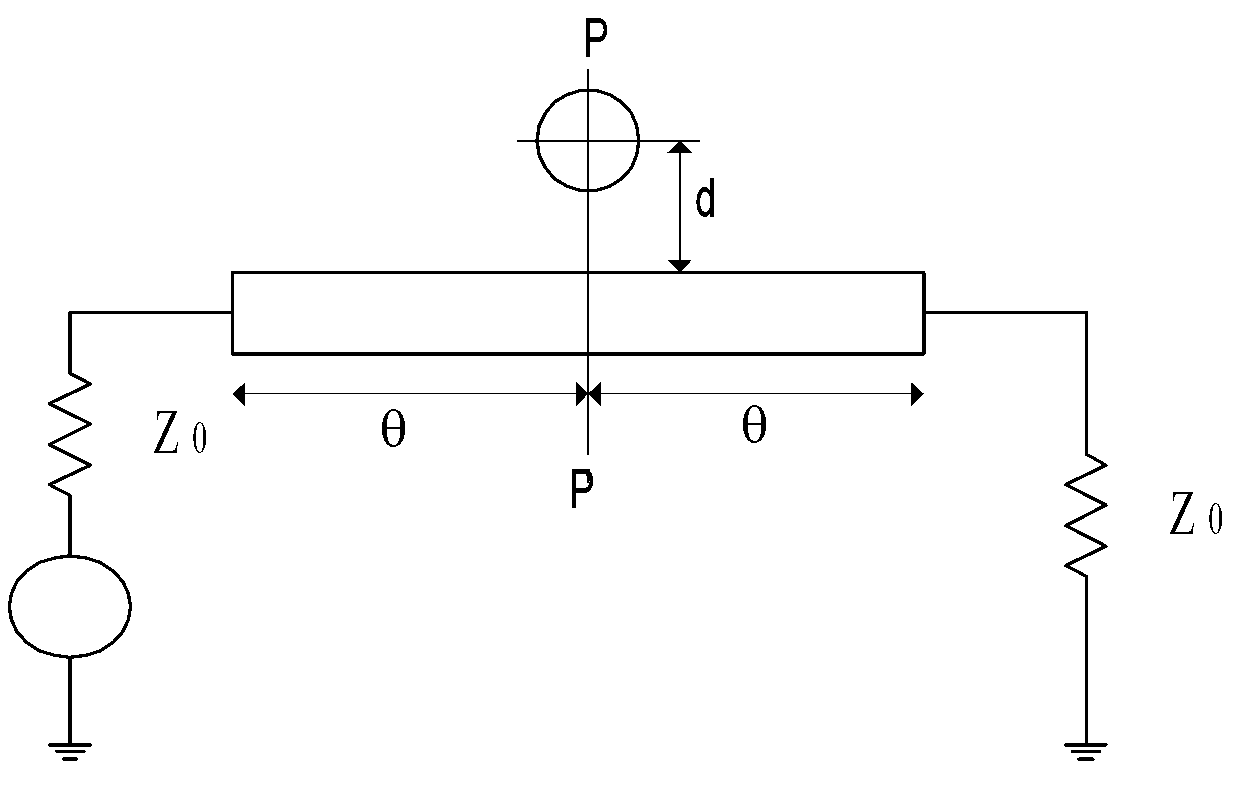
\includegraphics[width=3.8125in,height=2.4375in]{media/image2.png}

Equivalent electrical circuit is presented below:

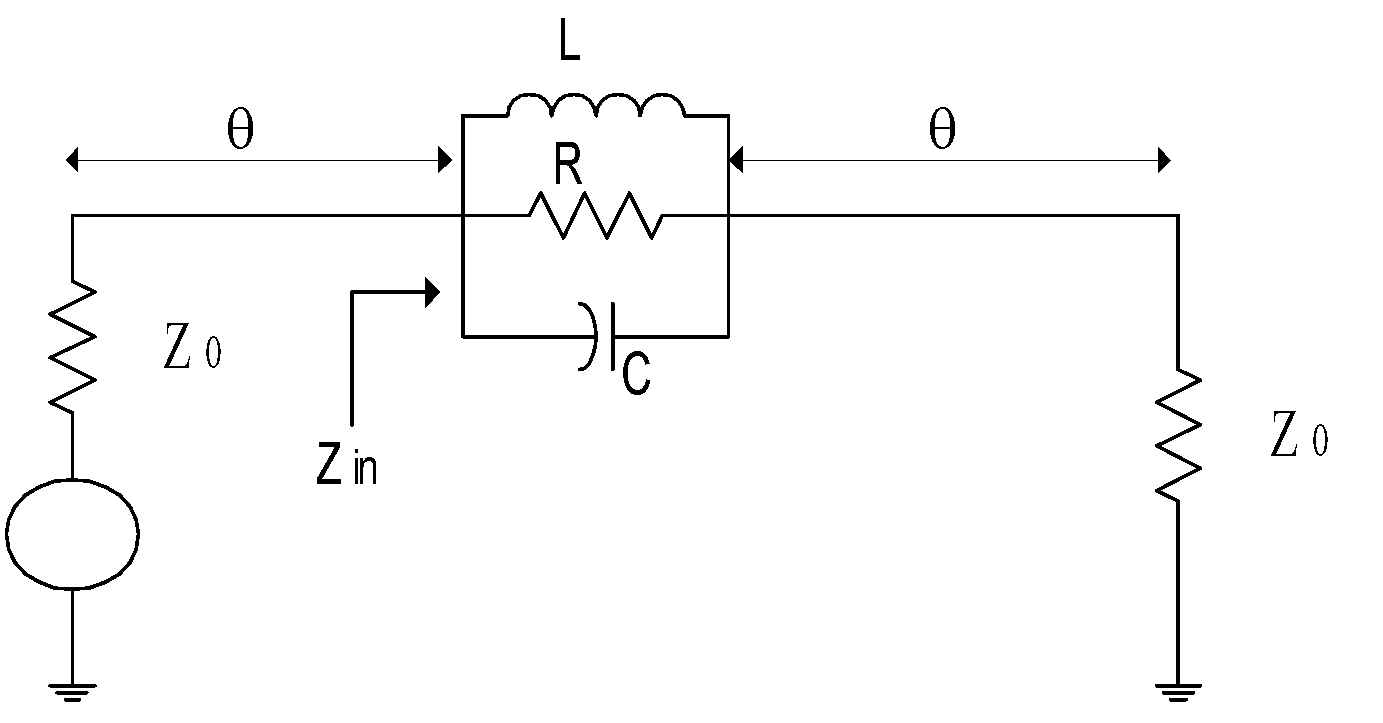
\includegraphics[width=3.88542in,height=2.03125in]{media/image3.png}

The coupling factor (\(k\)) between DR and transmission line is a
function of the distance (\(d\)) and is calculated as:

\[k = \frac{R}{R_{\text{ext}}} = \frac{R}{2Z_{0}} = \frac{S_{110}}{S_{210}}\]

\(S_{110}\)and \(S_{110}\) are the S-parameters in PP' plane at the
resonance frequency. Normalized input impedance is:

\[z_{\text{in}} = \frac{2k}{1 + 2\text{jQ}_{u}\delta} + 1\]

\[\delta = \frac{f - f_{0}}{f_{0}}\]

Where \(f_{0}\) is DR resonance frequency, \(f\) is operating frequency
and \(Q_{u}\) is an unloaded quality factor.

According to

\(S_{11} = \frac{z_{\text{in}} - 1}{z_{\text{in}} + 1}\);

and

\(S_{11} + S_{21} = 1\),

2-port S-parameter of the DR which is coupled with microstrip line, in
PP' plane will be:

\[\left\lbrack S_{R} \right\rbrack = \begin{bmatrix}
\frac{k}{k + 1 + 2\text{jQ}_{u}\delta} & \frac{1 + j2Q_{u}\delta}{k + 1 + 2\text{jQ}_{u}\delta} \\
\frac{1 + j2Q_{u}\delta}{k + 1 + 2\text{jQ}_{u}\delta} & \frac{k}{k + 1 + 2\text{jQ}_{u}\delta} \\
\end{bmatrix}\]

In resonance frequency \((f = f_{0})\) S-matrix will simplify to:

\[\left\lbrack S_{R_{0}} \right\rbrack = \begin{bmatrix}
\frac{k}{k + 1} & \frac{1}{k + 1} \\
\frac{1}{k + 1} & \frac{k}{k + 1} \\
\end{bmatrix}\]

The length of the transmission will impact S-parameter by:

\[\widehat{S_{\text{ij}}} = S_{\text{ij}}e^{- j2\theta}\]

It must be mentioned that the DR coupled microstrip line has bandstop
property. The line insertion loss is calculated from:

\[L_{0} = 20log(1 + k)\]

The coupling factor and the quality factors are related as below:

\[Q_{u} = Q_{L}(1 + k) = \text{kQ}_{e}\]

That \(Q_{u}\), \(Q_{L}\), \(Q_{e}\) are unloaded, loaded and external
quality factors. In the DR coupled microstrip line, these quality
factors and the coupling factor are calculated by measuring\(S_{11}\),
\(S_{21}\) using a network analyzer.

\begin{quote}
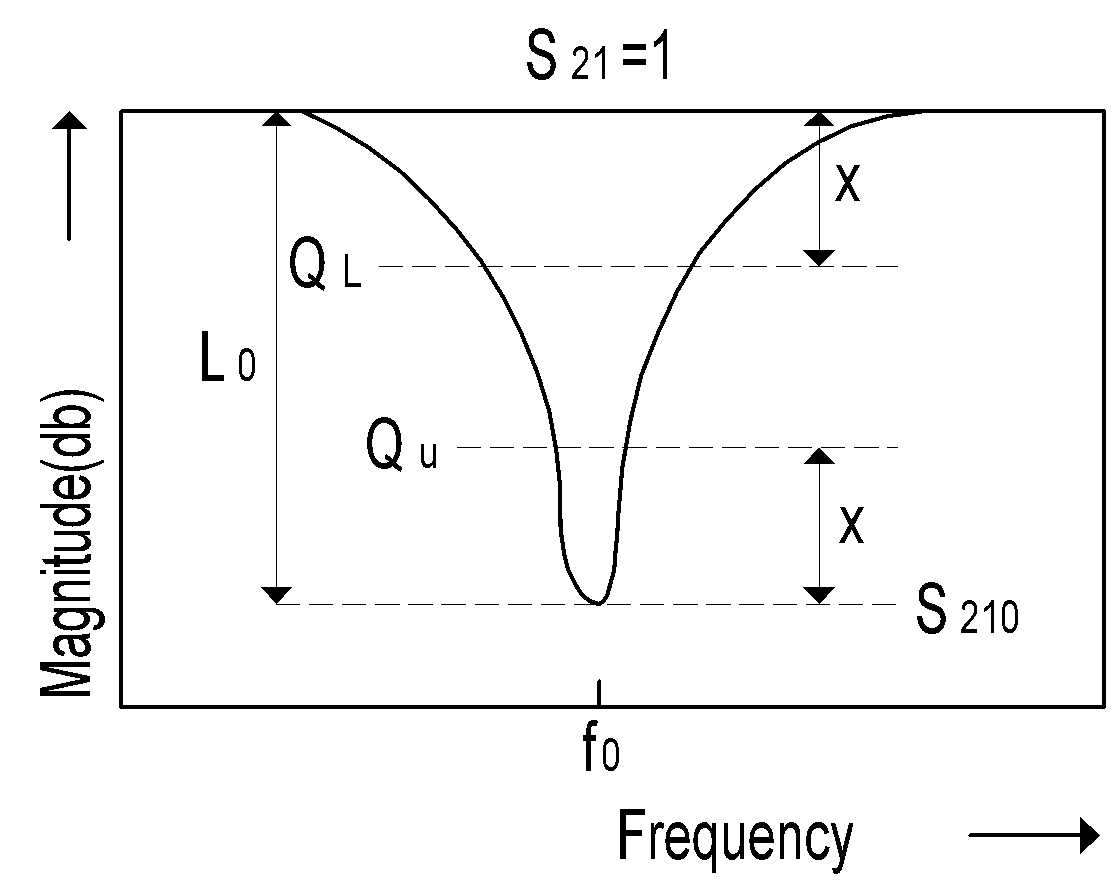
\includegraphics[width=2.68056in,height=2.15278in]{media/image4.png}
\end{quote}

\[L_{0}(dB) = 20logS_{210}\]

\[x(dB) = 3 - 10log(1 + 10^{- 0.1L_{0}})\]

\[k = 10^{\frac{L_{0}}{20}} - 1\]

Another possible configuration is that the DR to be coupled between two
microstrip lines, as shown in below which acts as a bandpass filter.

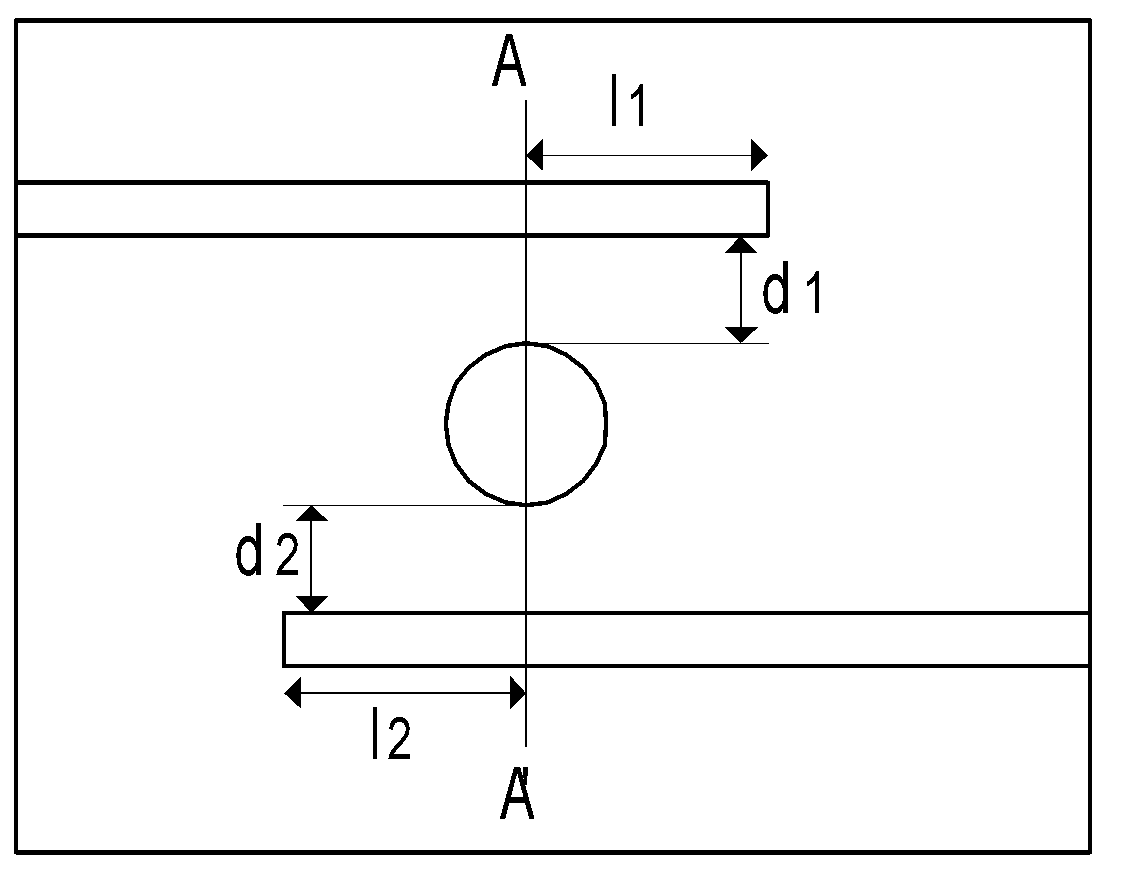
\includegraphics[width=2.61458in,height=2.05764in]{media/image5.png}

This configuration can be used to provide a parallel feedback loop in
TDROs, with equivalent circuit of:

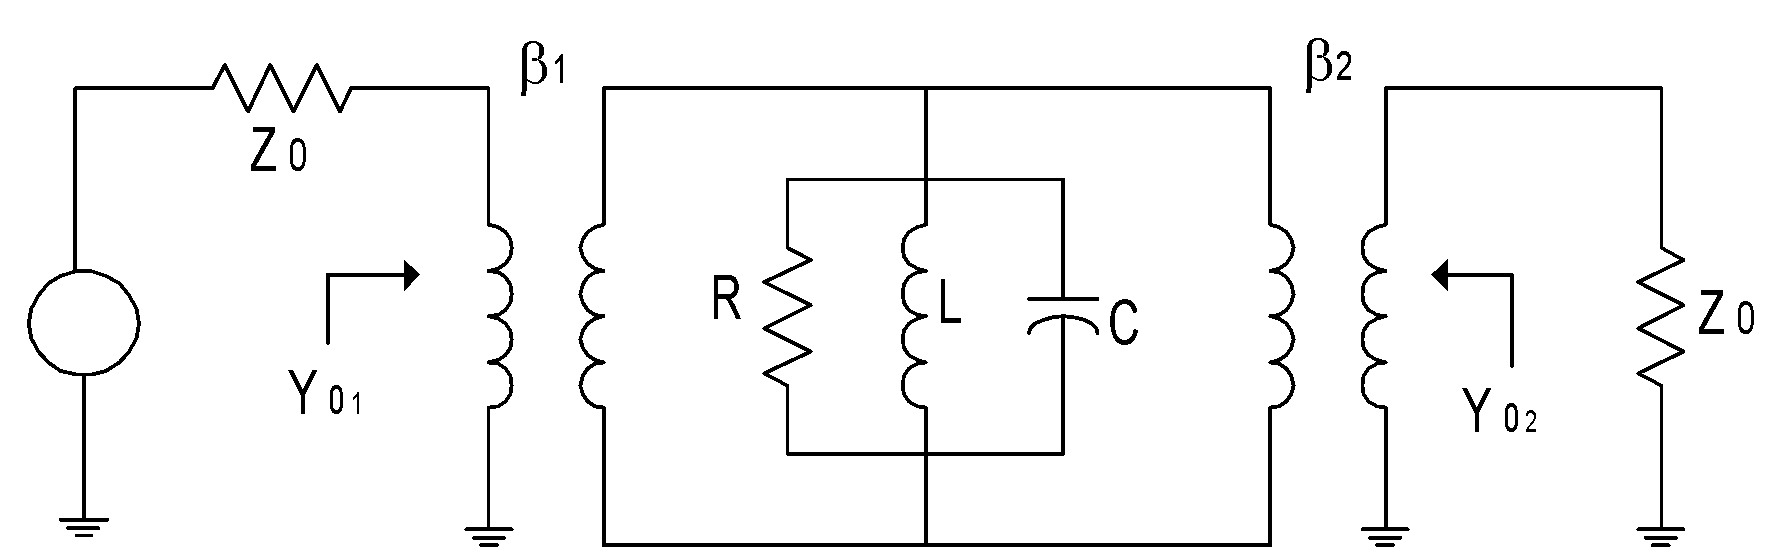
\includegraphics[width=4.83333in,height=1.51597in]{media/image6.png}

Note that to maximize magnetic coupling between microstrip line and DR,
lengths of l\textsubscript{1}, l\textsubscript{2}, needs to be quarter
of wavelength.

The S-matrix of this configuration in AA' plane is:

\[\left\lbrack S_{R} \right\rbrack = \begin{bmatrix}
\frac{k_{1} - k_{2} - 1 - j2Q_{u}\delta}{1 + k_{1} + k_{2} + j2Q_{u}\delta} & \frac{2k_{1}k_{2}}{1 + k_{1} + k_{2} + j2Q_{u}\delta} \\
\frac{2k_{1}k_{2}}{1 + k_{1} + k_{2} + j2Q_{u}\delta} & \frac{k_{1} - k_{2} - 1 - j2Q_{u}\delta}{1 + k_{1} + k_{2} + j2Q_{u}\delta} \\
\end{bmatrix}\]

where k\textsubscript{1}, k\textsubscript{2} are coupling factors
between DR and input and output transmission lines:

\[k_{1} = \frac{n_{1}^{2}R}{Z_{0_{1}}}\]

\[k_{2} = \frac{n_{2}^{2}\text{\ R}}{Z_{0_{2}}}\]

\[Q_{u} = Q_{L}(1 + k_{1} + k_{2})\]

\hypertarget{port-s-parameter-of-transistor}{%
\subsection{3 port S-parameter of
transistor}\label{port-s-parameter-of-transistor}}

While a transistor is a 3 port active element, the manufacturers always
provide a 2-port S-matrix; with the 3rd port (often Source or Emitter)
has been connected to ground. In circuit topologies that this 3rd port
remains connected to ground, the 2-port S parameter is sufficient.
However, for many different reasons, there are several circuit
configurations where the 3rd port is not connected to the ground.
Consequently, 3-port S-parameters need to be calculated from provided
2-port S-parameters. The details have been described in ``Foundation for
microwave engineering'' by R.E. Collin, where here only the final
results are mentioned.

\begin{quote}
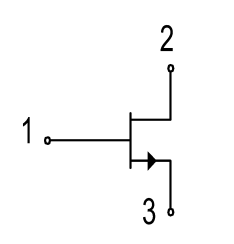
\includegraphics[width=1.0625in,height=1.10972in]{media/image7.png}
\end{quote}

\begin{longtable}[]{@{}lll@{}}
\toprule
\(\widehat{S_{11}} = S_{11} + \frac{s_{11}s_{12}}{4 - s}\) &
\(\widehat{S_{12}} = S_{12} + \frac{s_{11}s_{21}}{4 - s}\) &
\(\widehat{S_{13}} = \frac{2s_{11}}{4 - s}\)\tabularnewline
\midrule
\endhead
\(\widehat{S_{21}} = S_{21} + \frac{s_{22}s_{12}}{4 - s}\) &
\(\widehat{S_{22}} = S_{22} + \frac{s_{22}s_{21}}{4 - s}\) &
\(\widehat{S_{23}} = \frac{2s_{22}}{4 - s}\)\tabularnewline
\(\widehat{S_{31}} = \frac{2s_{12}}{4 - s}\) &
\(\widehat{S_{32}} = \frac{2s_{21}}{4 - s}\) &
\(\widehat{S_{33}} = \frac{2s}{4 - s}\)\tabularnewline
\bottomrule
\end{longtable}

and

\begin{longtable}[]{@{}ll@{}}
\toprule
\(s_{12} = 1 - S_{11} - S_{21}\) &
\(s_{11} = 1 - S_{11} - S_{12}\)\tabularnewline
\midrule
\endhead
\(s_{22} = 1 - S_{22} - S_{21}\) &
\(s_{21} = 1 - S_{22} - S_{12}\)\tabularnewline
\(s = 2 - s_{11} - s_{22}\) &\tabularnewline
\bottomrule
\end{longtable}

Where \(S_{\text{ij}}\) is 2-port and \(\widehat{S_{\text{ij}}}\) is 3
port S-parameter.

\hypertarget{oscillation-and-stability-conditions}{%
\subsection{Oscillation and Stability
conditions}\label{oscillation-and-stability-conditions}}

An oscillator circuit can be divided in 2 parts: Non-linear impedance
with negative real part Z\textsubscript{NL} and linear load impedance
Z\textsubscript{L}, assuming that, high Q of circuit will eliminate the
harmonics.

\begin{quote}
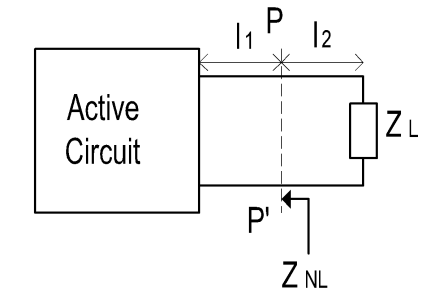
\includegraphics[width=1.95833in,height=1.375in]{media/image8.png}
\end{quote}

Electrical equivalent circuit is:

\begin{quote}
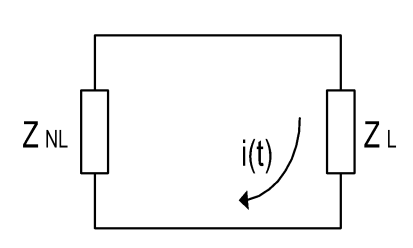
\includegraphics[width=1.875in,height=1.125in]{media/image9.png}
\end{quote}

Suppose that i(t) is sinusoidal:

\(i(t) = I_{0}cos(wt)\)

using Kirchhoff (\(\sum_{}^{}V = 0\)) law, in PP' plane:

\[\left\lbrack Z_{\text{NL}}(I_{0},w_{0}) + Z_{L}(w_{0}) \right\rbrack I_{0} = 0\]

if

\[Z_{\text{NL}} + Z_{L} = Z_{T} = R_{T} + \text{jX}_{T}\]

and knowing that:

\[\sum_{i = 1}^{3}S_{\text{ij}} = 1\ ;j = 1,2,3\]

If \(I_{0}\)is non-zero, then we must have:

\[R_{T}(I_{0},w_{0}) = 0\]

\[X_{T}(I_{0},w_{0}) = 0\]

Where

\[Re(Z_{L}) > 0\]

which means

\[Re(Z_{\text{NL}}) < 0\]

It implies the oscillation condition requires a negative real impedance.

The frequency of oscillation will be specified by
\(X_{T}(I_{0},w_{0}) = 0\)equation meaning the load reactance must be
equal and opposite of the active circuit reactance. In microwave
frequency, oscillating condition is normally written in term of
\(\Gamma_{L}\ \)and \(\Gamma_{\text{NL}}\) .

\[\left| \Gamma_{\text{NL}} \right| \cdot \left| \Gamma_{L} \right| = 1\]

\[\Gamma_{\text{NL}} + \Gamma_{L} = 2\pi\]

According to the amplitude condition of
\(\left| \Gamma_{\text{NL}} \right| \cdot \left| \Gamma_{L} \right| = 1\)
and knowing that \(\left| \Gamma_{L} \right| < 1\), we will find that
\(\left| \Gamma_{\text{NL}} \right|\) must be more than 1. An oscillator
has several active and passive parts where each is defined with its own
S-parameters. The circuit can be divided in two sections, active and
passive, like below:

\begin{quote}

\includegraphics[width=5.52778in,height=1.76389in]{media/image10.png}
\end{quote}

For active section:

\[\left\lbrack b \right\rbrack = \left\lbrack S \right\rbrack\left\lbrack a \right\rbrack\]

and passive section:

\[\left\lbrack b^{'} \right\rbrack = \left\lbrack S^{'} \right\rbrack\left\lbrack a^{'} \right\rbrack\]

based on the above figure;

\[\left\lbrack b \right\rbrack = \left\lbrack a^{'} \right\rbrack\]

we have:

\[\left\lbrack a^{'} \right\rbrack = \left\lbrack S \right\rbrack\left\lbrack S^{'} \right\rbrack\left\lbrack a^{'} \right\rbrack\]

or

\[\left( \left\lbrack S \right\rbrack\left\lbrack S^{'} \right\rbrack - \left\lbrack I \right\rbrack \right)\left\lbrack a^{'} \right\rbrack = \left\lbrack 0 \right\rbrack\]

Where {[}I{]} is the identity matrix. Unity matrix, {[}M{]}, is defined
as:

\[\left\lbrack M \right\rbrack = \left\lbrack S \right\rbrack\left\lbrack S^{'} \right\rbrack - \left\lbrack I \right\rbrack\]

If \(\left\lbrack a^{'} \right\rbrack \neq 0\), above condition becomes:

\[\det\left\lbrack M \right\rbrack = 0\]

which is a general term for large signal analyzing of oscillators.
However, for designing oscillators using small signal analysis the
condition of \(\det\left\lbrack M \right\rbrack = 0\) will transfer to:

\[\left| \det\left( \left\lbrack S \right\rbrack\left\lbrack S^{'} \right\rbrack - \left\lbrack I \right\rbrack \right) \right| > 0\]

and

\[\text{Arg}\left\{ \det\left( \left\lbrack S \right\rbrack\left\lbrack S^{'} \right\rbrack - \left\lbrack I \right\rbrack \right) \right\} = 0\]

If the above conditions are met, oscillation will start and amplitude of
oscillation will increase, until the active component becomes
non-linear. Moreover, the circuit gain decreases and reaches a steady
state. For example, consider the 2 port active circuit as below:

\begin{quote}
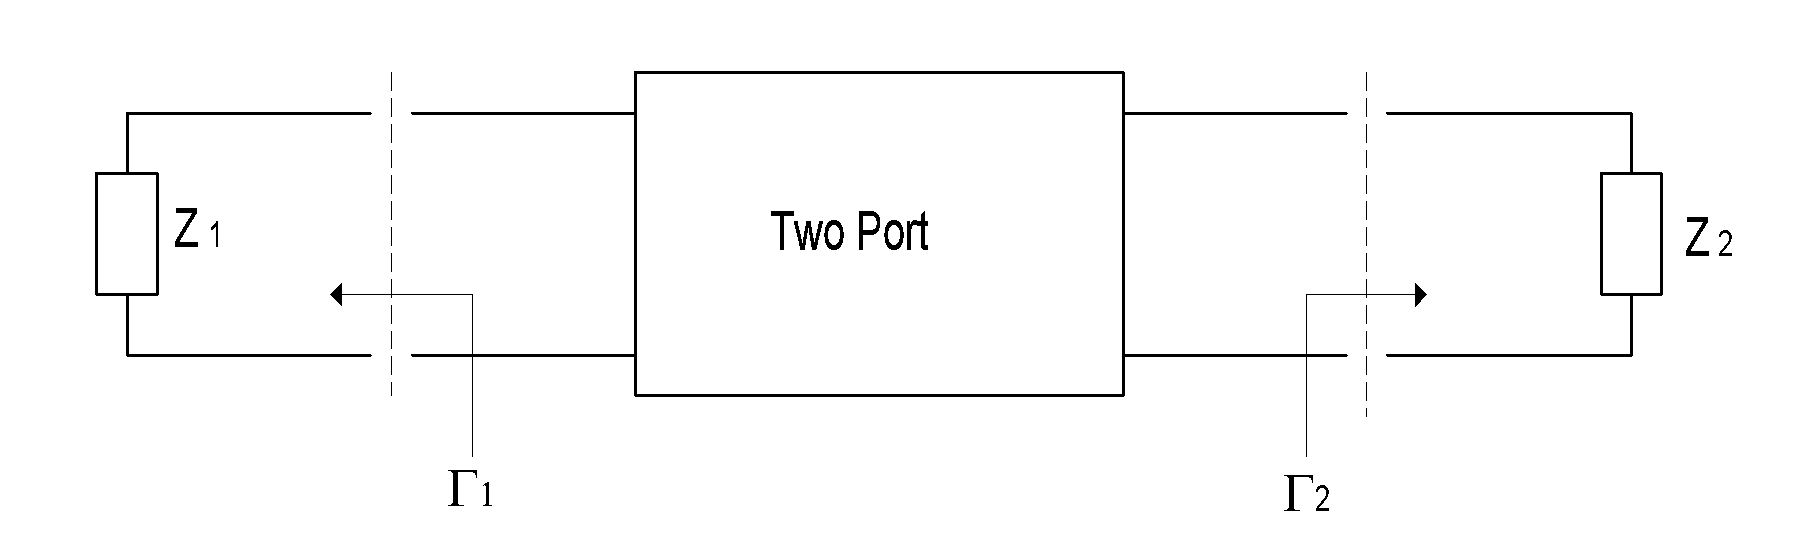
\includegraphics[width=5.52778in,height=1.70833in]{media/image11.png}
\end{quote}

and S-Parameter of the active element is:

\[\left\lbrack S \right\rbrack = \begin{bmatrix}
S_{\text{11}} & S_{\text{12}} \\
S_{\text{21}} & S_{\text{22}} \\
\end{bmatrix}\]

and the passive circuit is:

\[\left\lbrack S^{'} \right\rbrack = \begin{bmatrix}
\Gamma_{1} & 0 \\
0 & \Gamma_{2} \\
\end{bmatrix}\]

Oscillation condition, can be rewritten as:

\[\text{det}\left\lbrack M \right\rbrack = \text{det}\begin{bmatrix}
S_{\text{11}}\Gamma_{1} - 1 & S_{\text{12}}\Gamma_{2} \\
S_{\text{21}}\Gamma_{1} & S_{\text{22}}\Gamma_{2} - 1 \\
\end{bmatrix} = 0\]

which will result:

\[\left( S_{11}\Gamma_{1} - 1 \right)\left( S_{22}\Gamma_{2} - 1 \right) - S_{12}S_{21}\Gamma_{1}\Gamma_{2} = 0\]

Solving above results in two equations for the condition of oscillation:

\[S_{11} + \frac{S_{12}S_{21}\Gamma_{2}}{1 - S_{22}\Gamma_{2}} = \frac{1}{\Gamma_{1}}\]

\[S_{22} + \frac{S_{12}S_{21}\Gamma_{1}}{1 - S_{11}\Gamma_{1}} = \frac{1}{\Gamma_{2}}\]

\hypertarget{stabilizing-oscillators}{%
\subsection{Stabilizing Oscillators}\label{stabilizing-oscillators}}

An oscillator is stable, when changes to RF voltages and currents from
its operating point are damped rapidly, and the oscillator returns to
its original condition. Analyzing stability of an oscillator, using
Quasi-Static estimation, a small change in I\textsubscript{0} is
introduced, and the response of the circuit to this change will be
analyzed. The change to the current amplitude (\(\text{δI}_{0}\)), in
PP' plane results:

\[Z_{T}\left( I_{0}{,w}_{0} \right) + \frac{{\partial Z}_{T}}{\partial p}\delta p + \frac{{\partial Z}_{T}}{\partial I_{0}}{\delta I}_{0} = 0\]

with assumption of:

\[Z_{T}\left( I_{0},w_{0} \right) = 0\]

then:

\[\delta p = - j\frac{\frac{{\delta Z}_{T}}{{\delta I}_{0}} \cdot \frac{\delta Z_{T}^{*}}{\delta w}}{\left| \frac{{\delta Z}_{T}}{\delta w} \right|^{2}} \cdot {\delta I}_{0}\]

\(\delta\)p can be divided into real and imaginary parts:

\[\delta p = \alpha + j\delta w\]

The oscillator will be stable, if the real part (\(\alpha\)) decreases
as current amplitude is increased. It translates to:

\[\frac{{\delta R}_{T}}{{\delta I}_{0}} \cdot \frac{{\delta X}_{T}}{\delta w} - \frac{{\delta X}_{T}}{{\delta I}_{0}} \cdot \frac{{\delta R}_{T}}{\delta w} > 0\]

which is the stability condition of the oscillator for amplitude of
I\textsubscript{0} and angular frequency of jw. For imaginary part of δw
to be sufficiently small, using
\(\text{δp} = - j\frac{\frac{\text{δZ}_{T}}{\text{δI}_{0}} \cdot \frac{\delta Z_{T}^{*}}{\text{δw}}}{\left| \frac{\text{δZ}_{T}}{\text{δw}} \right|^{2}} \cdot \text{δI}_{0}\),
the below condition must be met:

\[\frac{{\delta R}_{T}}{{\delta I}_{0}} \cdot \frac{{\delta R}_{T}}{\delta w} + \frac{{\delta X}_{T}}{{\delta I}_{0}} \cdot \frac{{\delta X}_{T}}{\delta w} = 0\]

If the above condition is met, the changes of δI\textsubscript{0}, will
not result in a change of oscillation frequency.

\hypertarget{selecting-circuit-components}{%
\section{Selecting circuit
components}\label{selecting-circuit-components}}

The designing method that will be explained later can be applied to BJT
or FET, and is based on semiconductor small signal S-parameters. For
designing a stable oscillator, a DR can be used in different
configurations:

\begin{enumerate}
\def\labelenumi{\arabic{enumi}.}
\item
  As a passive element is coupled with a free-run oscillator;
\item
  As one of the elements (e.g. in feedback, matching network) of
  oscillator circuit, to specify oscillation frequency.
\end{enumerate}

Passive stability can only be used on a free-run oscillator that its
frequency of oscillation is dependent on load impedance. When the
oscillating frequency is established, any deviation will cause a
relatively big change in load impedance, causing the oscillating
frequency to return to its original. In this kind of oscillators, DR
electrical distance (θ) to the output of oscillator circuit is between
generally \(\frac{\lambda_{g}}{4}\) and \(\frac{\lambda_{g}}{2}\).

\begin{quote}
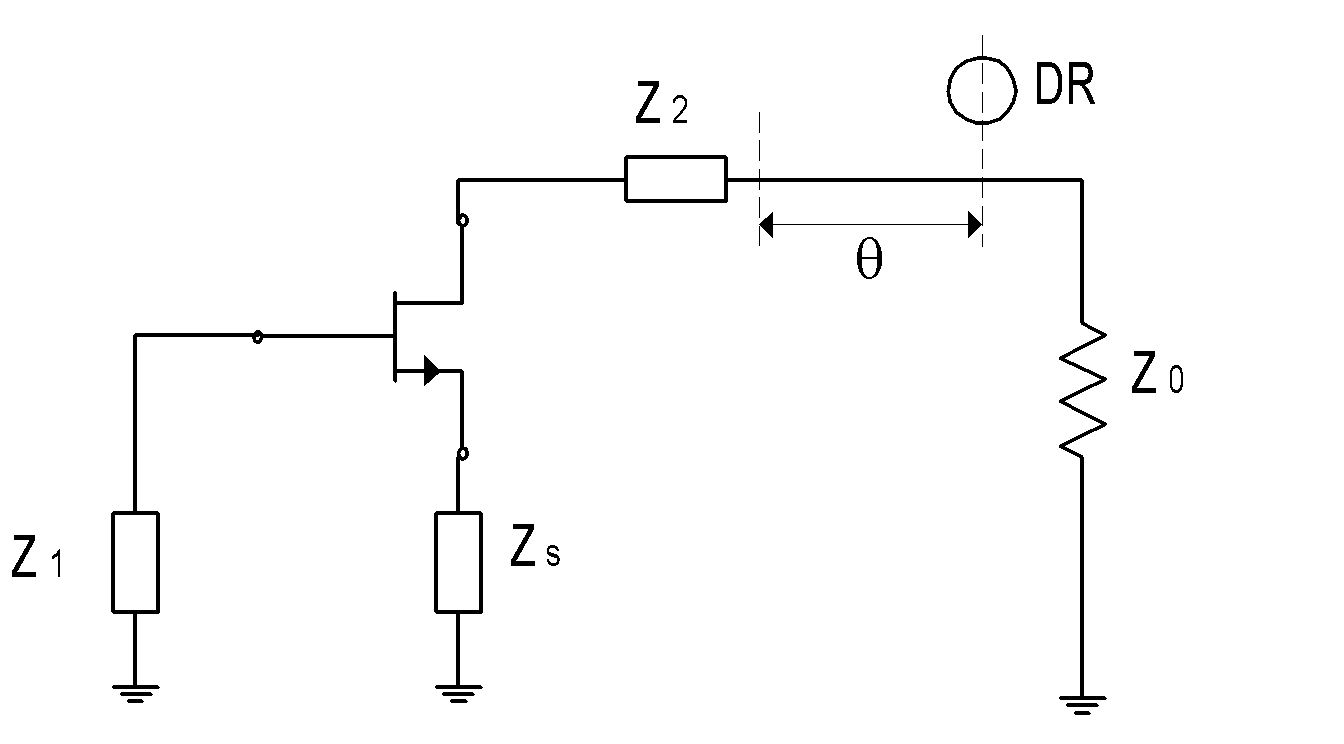
\includegraphics[width=3.76389in,height=2.08333in]{media/image12.png}
\end{quote}

Suppose that \(\theta = \pi\) (one-half of wavelength), using
\(z = \frac{2k}{1 + 2\text{jQ}_{u}\delta} + 1\) normalized input
admittance of DR is:

\[Y_{\text{in}} = \frac{1}{1 + \frac{2k}{1 + jD}}\]

where

\[D = 2Q_{u}\delta\]

real and imaginary parts of admittance are:

\[\text{Re}\left( Y_{\text{in}} \right) = \frac{1 + 2k + D^{2}}{\left( 1 + 2k \right)^{2} + D^{2}}\]

\[\text{Im}\left( Y_{\text{in}} \right) = \frac{2kD}{\left( 1 + 2k \right)^{2} + D^{2}}\]

To calculate the stabilized frequency range \(\delta_{f}\), the first
derivative of imaginary of admittance to the frequency needs to be zero:

\[\frac{\text{dB}}{\text{df}} = \frac{4Q_{u}\left\lbrack \left( 1 + 2k \right)^{2} - D^{2} \right\rbrack}{f_{0}\left\lbrack \left( 1 + 2k \right)^{2} + D^{2} \right\rbrack} = 0\]

which results to:

\[D = \pm \left( 1 + 2k \right)\]

or

\[\delta_{f} = \pm \frac{f_{0}}{2Q_{u}}\left( 1 + 2k \right)\]

Bandwidth, \(\delta_{s} = 2\delta_{f}\), based on the reflection
coefficient S\textsubscript{210} and S\textsubscript{110}, will be:

\[\delta_{s} = \frac{f_{0}}{Q_{u}}\left( \frac{1 + S_{110}}{S_{210}} \right)\]

This method of stabilizing oscillators, will decrease output power for
two reasons:

\begin{enumerate}
\def\labelenumi{\arabic{enumi}.}
\item
  Output power of free-run oscillators depends on load impedance
  Y\textsubscript{L} and it will maximize for Re(YL)=1. At oscillation
  frequency we have
  \(\text{Re}\left( Y_{L} \right) = \frac{1}{1 + 2k} = \frac{S_{210}}{1 + S_{110}}\)
  which decreases the output power by
  \(L_{1} = P_{0}\left( \frac{\left( \frac{Y_{0}S_{210}}{1 + S_{110}} \right)}{P_{0}\left( Y_{0} \right)} \right)\)
\item
  The insertion loss of DR (S\textsubscript{210}) will decrease the
  output power by
  \(L_{2} = \frac{1}{\left( 1 + k \right)^{2}} = \frac{1}{S_{210}^{2}\ }\)
\end{enumerate}

The total insertion loss will be the sum of two above insertion loss
(L\textsubscript{1}, L\textsubscript{2}).

This stability method has multiple disadvantages. The presence of two
resonant circuits (tank circuit of free-run oscillator and DR) can cause
multiple modes resulting in hysteresis and unstable frequency of
operation. However, if designed carefully, it is a less complex method,
making the circuit and tuning it easier. In the rest of this thesis,
this method for stabilization has been used.

\hypertarget{choosing-the-components}{%
\subsection{Choosing the components}\label{choosing-the-components}}

The following selection of components is based on the target frequency
of 10GHz.

\hypertarget{substrate}{%
\subsubsection{\texorpdfstring{
Substrate}{ Substrate}}\label{substrate}}

The substrate must have a low loss tangent at the frequency of
operation. Based on the available materials, the following substrate has
been selected:

\begin{quote}
PTFE \(\epsilon_{r} = 2.33\) \({h = 0.031}^{''}\) \(t = 17.5m\)

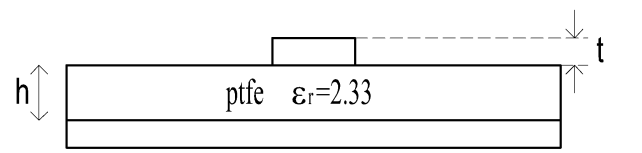
\includegraphics[width=2.91667in,height=0.69444in]{media/image13.png}
\end{quote}

\hypertarget{dielectric-resonator}{%
\subsubsection{\texorpdfstring{ Dielectric
Resonator}{ Dielectric Resonator}}\label{dielectric-resonator}}

Usually selecting DR requires studying the manufacturer's datasheets for
the operating frequencies and selecting DR that its resonant frequency
is the closest to the target oscillation frequency. However, in this
project, the circuit must be designed using an already specified DR and
use a technique to tune its resonant frequency. To tune DR resonant
frequency, after mounting DR on the substrate, a conductor plane on the
top of the DR is mounted using an adjustable screw. Changing the gap
between the conductor plane and the top of the DR, tunes its resonance
frequency, however, it will decrease Q. DR characteristics are as below:

εr=39 Hd=2.38mm D=5.9mm

\hypertarget{active-component}{%
\subsubsection{\texorpdfstring{ Active
component}{ Active component}}\label{active-component}}

For making a TDRO in X band, we can use both BJT and GaAs FET, here GaAs
FET NE71083 has been selected because its S-parameters at the frequency
of operation is available.

\hypertarget{microwave-simulation-software}{%
\subsubsection{\texorpdfstring{ Microwave simulation
software}{ Microwave simulation software}}\label{microwave-simulation-software}}

Based on the availability of three microwave simulation softwares; PUFF,
TouchStone and Super Compact and their parts library, Super
Compact\footnote{Version 6.0 of Super-Compact PC, Microwave Harmonica PC
  and Scope PC for Windows Links to Serenade. (1993, November 1).} has
been selected.

\hypertarget{tdro-design}{%
\section{TDRO design}\label{tdro-design}}

\hypertarget{port-s-parameter-of-ne71083}{%
\subsection{3 port S-parameter of
NE71083}\label{port-s-parameter-of-ne71083}}

NEC NE71083 datasheet has 2 port S-parameters however it was previously
mentioned that a 3 port S-parameters is needed for designing an
oscillator. For calculating 3 port S-parameters, we will use 2 to 3 port
transformation as part of `Super Compact' software. It is only
sufficient to define a 3 node component for a `TWO' element and use the
same data of 2 port S-parameters. The software will perform the
necessary transformations.

\begin{longtable}[]{@{}l@{}}
\toprule
\endhead
\begin{minipage}[t]{0.97\columnwidth}\raggedright
\begin{quote}
BLK\\
TWO 1 2 3 NE71083\\
THREE:3POR 1 2 3\\
END\\
~\\
FREQ\\
STEP 2GHz 18GHz 200MHz\\
END\\
~\\
OUT\\
PRI THREE S\\
END\\
~\\
DATA\\
~\\
NE71083: S ;Data for NE71083 GaAs MESFET\\
~\\
2GHZ .95 -26 3.54 161 .04 79 .59 -13\\
4GHZ .89 -50 3.1 141 .06 66 .58 -24\\
6GHZ .82 -70 2.83 126 .08 56 .54 -33\\
8GHZ .78 -80 2.49 114 .09 51 .5 -42\\
10GHZ .73 -102 2.15 104 .1 48 .47 -48\\
12GHZ .71 -114 1.95 93 .1 43 .45 -55\\
14GHZ .71 -122 1.93 90 .11 44 .47 -62\\
16GHZ .67 -128 1.64 76 .11 43 .49 -64\\
18GHZ .66 -140 1.47 63 .11 40 .52 -70\\
~\\
END
\end{quote}\strut
\end{minipage}\tabularnewline
\bottomrule
\end{longtable}

\hypertarget{calculating-width-of-the-microstrip-line}{%
\subsection{\texorpdfstring{ Calculating width of the microstrip
line}{ Calculating width of the microstrip line}}\label{calculating-width-of-the-microstrip-line}}

A 50Ω microstrip is calculated to be 2.31mm wide, using the `Super
Compact' TRL tool.

\hypertarget{circuit-configuration}{%
\subsection{\texorpdfstring{ Circuit
Configuration}{ Circuit Configuration}}\label{circuit-configuration}}

As described before to reduce the complexity of design, build and tuning
the following circuit configuration has been selected:

\begin{quote}
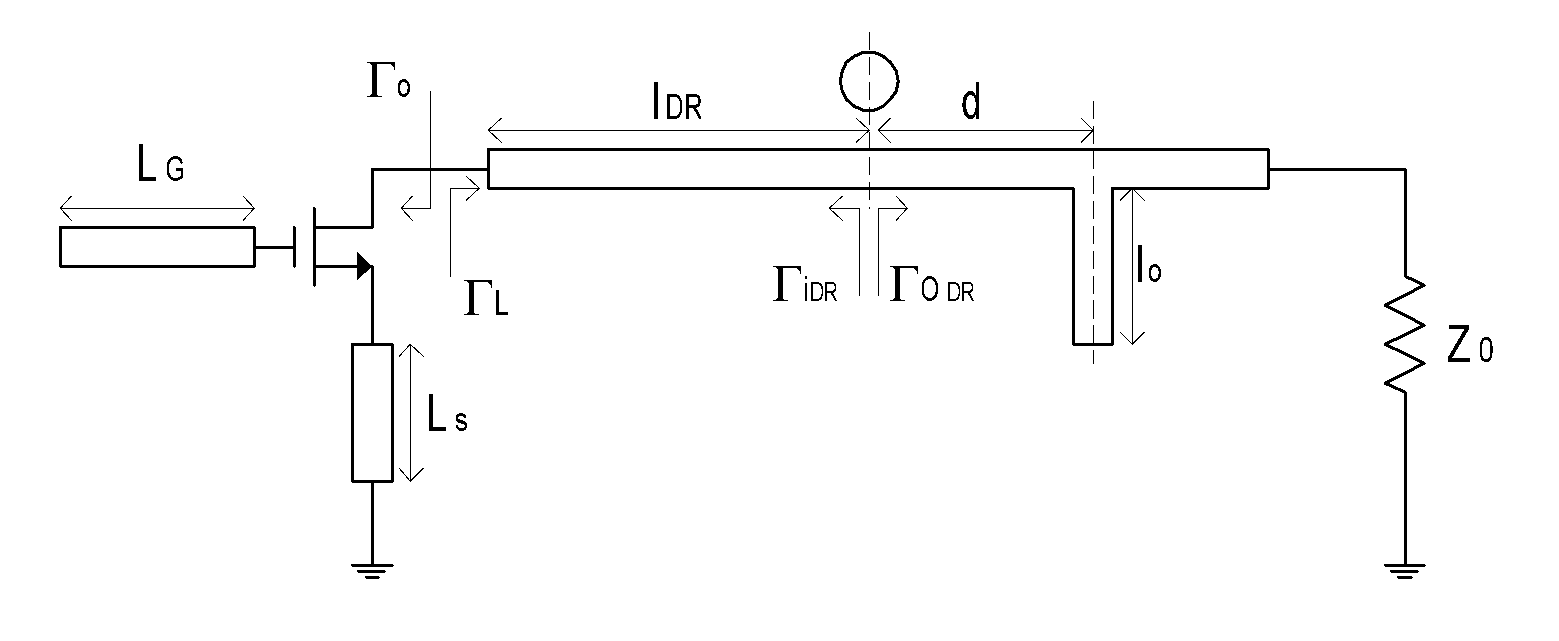
\includegraphics[width=5in,height=2.05556in]{media/image14.png}
\end{quote}

L\textsubscript{G} and L\textsubscript{S} are selected so at the
operating frequency is \(2 \leq \left| \Gamma_{o} \right| \leq 4\) and
in other frequencies \(\left| \Gamma_{o} \right| < 1\). Maximizing the
slope of the Γo-f curve will improve the condition of oscillation.
L\textsubscript{G} and L\textsubscript{S} are calculated using the
following circuit file.

\begin{longtable}[]{@{}l@{}}
\toprule
\endhead
\begin{minipage}[t]{0.97\columnwidth}\raggedright
\begin{quote}
LS:?0 5.69mm 10mm?\\
LG:?0 9.5mm 12mm?\\
~\\
BLK\\
OST 1 W=2.31mm P=LG F=10GHz MSUB\\
TWO 1 2 3 NE71083\\
SST 3 W=2.31mm P=LS F=10GHz MSUB\\
~\\
OUT:1POR 2\\
END\\
~\\
FREQ\\
STEP 2GHz 18GHz 200MHz\\
END\\
~\\
OUT\\
PRI OUT S\\
END\\
~\\
OPT\\
OUT\\
F=10GHz\\
MS11=4 LT\\
MS11=2 GT\\
F=2GHz 10GHz\\
MS11=1 LT\\
F=10GHz 18GHz\\
MS11=1 LT\\
END\\
~\\
DATA\\
~\\
MSUB : MS ER=2.33 H=0.031in MET1=CU 17.5um\\
~\\
NE71083: S ;Data for NE71083 GaAs MESFET\\
~\\
2GHZ .95 -26 3.54 161 .04 79 .59 -13\\
4GHZ .89 -50 3.1 141 .06 66 .58 -24\\
6GHZ .82 -70 2.83 126 .08 56 .54 -33\\
8GHZ .78 -80 2.49 114 .09 51 .5 -42\\
10GHZ .73 -102 2.15 104 .1 48 .47 -48\\
12GHZ .71 -114 1.95 93 .1 43 .45 -55\\
14GHZ .71 -122 1.93 90 .11 44 .47 -62\\
16GHZ .67 -128 1.64 76 .11 43 .49 -64\\
18GHZ .66 -140 1.47 63 .11 40 .52 -70\\
~\\
END
\end{quote}\strut
\end{minipage}\tabularnewline
\bottomrule
\end{longtable}

which results to LG=9.5mm and LS=5.67mm and

\[\Gamma_{o} = 3.879 < - 12.638^{o}\]

To meet the oscillating condition, we must have:

\[\Gamma_{L} \geq \frac{1.3}{\Gamma_{o}}\]

A small signal correction factor of `1.3' is included into the
calculation to add margin of safety because the circuit is designed
using small signal S-parameters while the oscillator is non-linear. It
results to:

\[\Gamma_{L} = 0.3351 < 12.638^{o}\]

\hypertarget{placement-of-dr}{%
\subsection{\texorpdfstring{ Placement of
DR}{ Placement of DR}}\label{placement-of-dr}}

For optimal coupling between a microstrip line and DR, DR must be placed
where the maximum current/minimum voltage occurs on the line. To do so,
using a Smith Chart, move from Γ\textsubscript{L} to load on a constant
S circle, to reach the minimum voltage. Which means:

\[2\text{βl}_{\text{DR}} = 180 - 12.638\]

After populating the lines' parameters, it results:

\[l_{\text{DR}} = 0.233\lambda_{g}\]

According to substrate characteristics and its 50 Ω impedance

\[\lambda_{g} = 21.208mm\]

so:

\[l_{\text{DR}} = 4.93mm\]

because \(l_{\text{DR}} < \frac{\text{DR\ diameter}}{2}\), for omitting
evanescent modes, we add \(\frac{\lambda_{g}}{2}\) to \(l_{\text{DR}}\):

\[l_{\text{DR}} = 15.53mm\]

\hypertarget{gap-between-the-conductor-plane-and-top-of-dr}{%
\subsection{\texorpdfstring{ Gap between the conductor plane and top of
DR}{ Gap between the conductor plane and top of DR}}\label{gap-between-the-conductor-plane-and-top-of-dr}}

According to DR characteristics, calculating its resonant frequency
using Super Compact shows that its resonant frequency is far from 10GHz.
Optimizing for 10GHz resonant frequency, the gap between the top of DR
and the conductor place results in a 0.88mm gap and the microstrip line
to DR gap of 2.5mm. It's 2 port S-parameter at 10GHz is equal:

\[\left\lbrack S \right\rbrack = \begin{bmatrix}
0\text{.937<-}\text{20}^{o} & 0\text{.339} < \text{70}^{o} \\
0\text{.339} < \text{70}^{o} & 0\text{.937<-}\text{20}^{o} \\
\end{bmatrix}\]

Output Γ could be calculated:

\[\Gamma_{O_{\text{DR}}} = \frac{S_{11} - \left( S_{11}^{2} - S_{21}^{2} \right)\Gamma_{i_{\text{DR}}}}{1 - S_{11}\Gamma_{i_{\text{DR}}}}\]

\[\Gamma_{i_{\text{DR}}} = 0.3351 < 180^{o}\]

\[\Gamma_{O_{\text{DR}}} = 0.9656 < - 20.464^{o}\]

Now it's enough to match \(\Gamma_{O_{\text{DR}}}\) to 50Ω. For the
simplicity, a single-stub matching method is used:

\[d = 0.06\lambda_{g}\]

\[l_{o} = 0.026\lambda_{g}\]

And because

\[\lambda_{g} = 21.208mm\]

The matching becomes:

\[d = 1.27mm\]

\[l_{o} = 0.55mm\]

and results the following circuit:

\begin{quote}
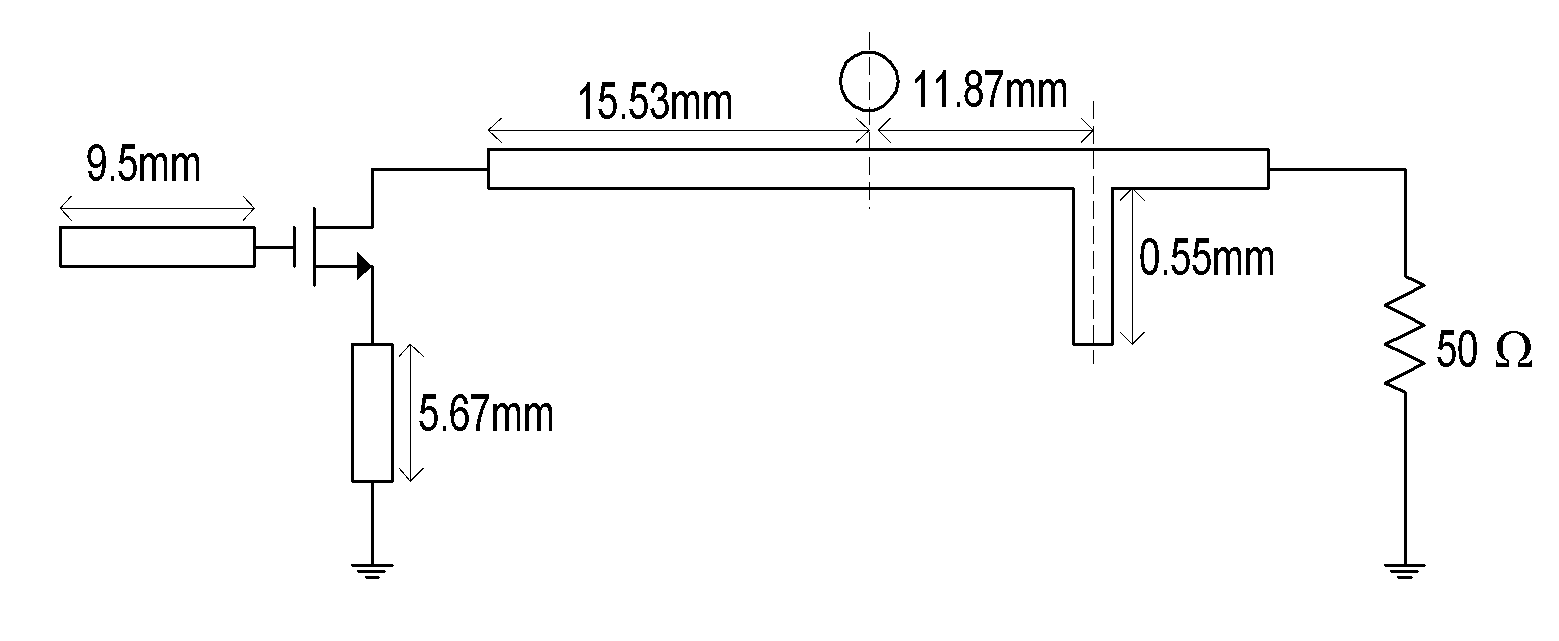
\includegraphics[width=5in,height=2.05556in]{media/image15.png}
\end{quote}

represented in Super Compact circuit as:

\begin{longtable}[]{@{}l@{}}
\toprule
\endhead
\begin{minipage}[t]{0.97\columnwidth}\raggedright
\begin{quote}
LDR:4.77MM\\
LT:?11.87MM?\\
~\\
BLK\\
OST 1 W=2.31MM P=9.37MM MSUB\\
TWO 1 2 3 NE71083\\
SST 3 W=2.31MM P=5.67MM MSUB\\
TRL 2 4 W=2.31MM P=(LDR-(LT-10.6MM)) MSUB\\
DRMS 4 5 D=5.9MM HD=2.38MM ER=39 S=2.5MM HT=?.8762MM? W=2.31MM L=LT BSF
MSUB\\
TEE 5 6 7 W1=2.31MM W2=2.31MM W3=2.31MM MSUB\\
OST 7 W=2.31MM P=?1.63MM? MSUB\\
OSC:1POR 6\\
END\\
~\\
FREQ\\
STEP 2GHZ 15GHZ 200MHZ\\
END\\
~\\
OUT\\
PRI OSC S\\
END\\
~\\
OPT\\
OSC F=10GHZ MS11 W=-1\\
OSC F=9.99GHZ 9.9999GHZ MS11\\
OSC F=10.0001GHZ 10.01GHZ MS11\\
END\\
~\\
DATA\\
~\\
MSUB : MS ER=2.33 H=0.031IN MET1=CU 17.5UM\\
~\\
NE71083: S ;Data for NE71083 GaAs MESFET\\
~\\
2GHZ .95 -26 3.54 161 .04 79 .59 -13\\
4GHZ .89 -50 3.1 141 .06 66 .58 -24\\
6GHZ .82 -70 2.83 126 .08 56 .54 -33\\
8GHZ .78 -80 2.49 114 .09 51 .5 -42\\
10GHZ .73 -102 2.15 104 .1 48 .47 -48\\
12GHZ .71 -114 1.95 93 .1 43 .45 -55\\
14GHZ .71 -122 1.93 90 .11 44 .47 -62\\
16GHZ .67 -128 1.64 76 .11 43 .49 -64\\
18GHZ .66 -140 1.47 63 .11 40 .52 -70\\
~\\
END
\end{quote}\strut
\end{minipage}\tabularnewline
\bottomrule
\end{longtable}

After Super Compact optimization, the circuit becomes:

\begin{quote}
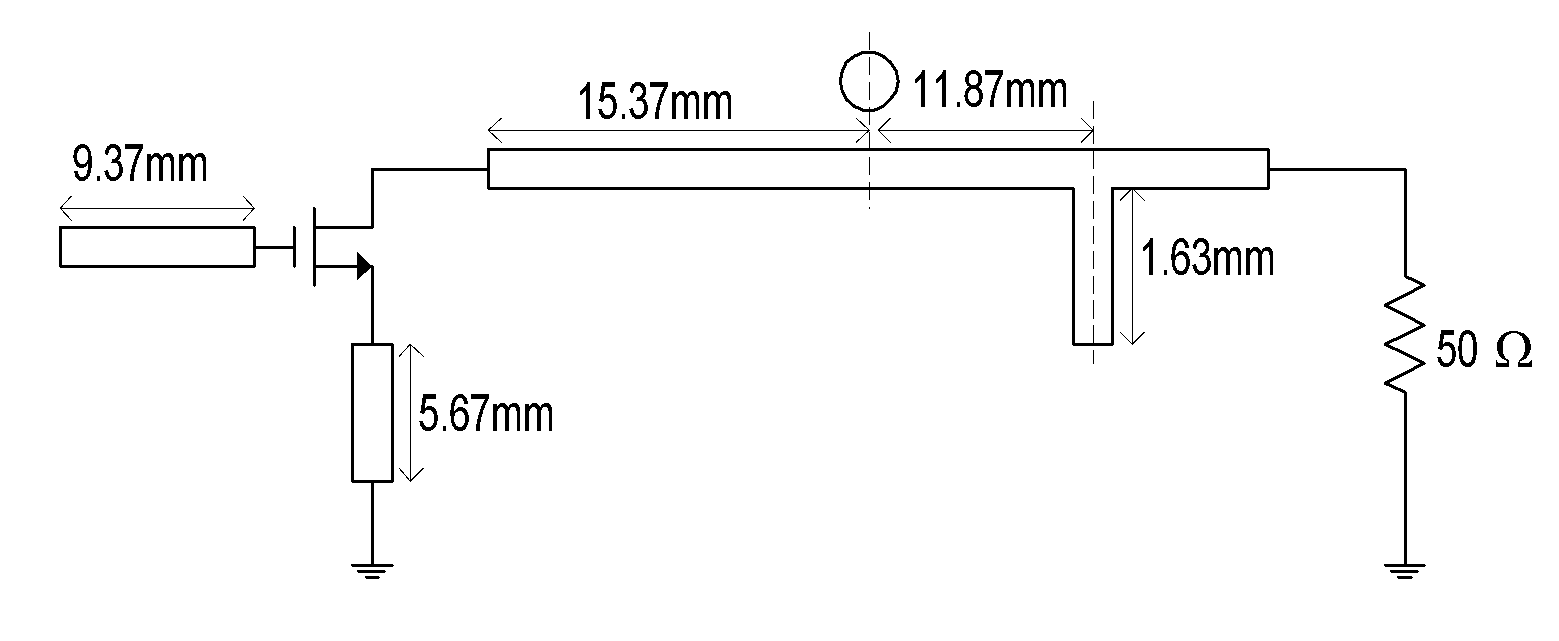
\includegraphics[width=5in,height=2.05556in]{media/image16.png}
\end{quote}

\hypertarget{dc-bias-circuit}{%
\subsection{\texorpdfstring{ DC bias
circuit}{ DC bias circuit}}\label{dc-bias-circuit}}

The DC bias circuit must not change the equivalent AC circuit. In order
to achieve that, the following need to be satisfied:

\begin{enumerate}
\def\labelenumi{\arabic{enumi}.}
\item
  Separate DC bias using RFC lines which have maximum feasible line
  impedance for the PCB technology; in our case \textasciitilde120Ω
  microstrip lines, from the AC circuit.
\item
  These RFC lines must be connected to the transmission lines at their
  minimum voltage location which maximize differences in impedances. It
  will minimize the impact of RFC lines on the AC circuit.
\item
  Use quarter wavelength for the RFC line and have one end of the RFC
  lines connected to AC ground using bypass capacitors. This will assure
  that the impedance seen at the other end of RFC lines are as large as
  possible.
\end{enumerate}

For Z\textsubscript{0}=120Ω, RFC line width will be 0.3mm. Also
previously, it is calculated that:

\[\lambda_{g} = 22.3mm\]

resulting RFC length to be:

\[l_{\text{RFC}} = \frac{\lambda_{g}}{4} = 5.58mm\]

The updated circuit is shown below, after optimizing by Super Compact.

A very \textbf{important note}, at the time of this project, the 10pF
bypass capacitors have self resonance of 2GHz corresponding to self
inductance of 0.47nH, which is added to the Super Compact circuit.

\begin{longtable}[]{@{}l@{}}
\toprule
\endhead
\begin{minipage}[t]{0.97\columnwidth}\raggedright
\begin{quote}
WB:0.3MM \#ND 0.01MM\#\\
WL:2.31MM \#ND 0.01MM\#\\
~\\
*ByPass information\\
CBY:10PF\\
LBY:0.478NH\\
~\\
BLK\\
* Gate Circuit\\
OST 1 W=WL P=4.9MM \#ND 0.01MM\# MSUB\\
TEE 1 2 3 W1=WL W2=WL W3=WB MSUB\\
~\\
VIA 31 D=1MM MSUB\\
TRL 31 32 W=2MM P=2MM MSUB\\
SRX 32 33 R=0 L=LBY C=CBY\\
TRL 33 34 W=1MM P=0.5MM MSUB\\
STEP 34 35 W1=1MM W2=0.3MM MSUB\\
TRL 35 3 W=0.3MM P=3.32MM MSUB\\
~\\
~\\
TRL 2 4 W=WL P=4.31MM \#ND 0.01MM\# MSUB\\
~\\
TWO 4 5 6 NE71083\\
~\\
* Source Circuit\\
SST 6 W=WL P=5.67MM \#ND 0.01MM\# MSUB\\
~\\
* Drain Circuit\\
TRL 5 7 W=WL P=4.86MM \#ND 0.01MM\# MSUB\\
TEE 7 8 9 W1=WL W2=WL W3=WB MSUB\\
~\\
VIA 91 D=1MM MSUB\\
TRL 91 92 W=2MM P=2MM MSUB\\
SRX 92 93 R=0 L=LBY C=CBY\\
TRL 93 94 W=1MM P=0.5MM MSUB\\
STEP 94 95 W1=1MM W2=0.3MM MSUB\\
TRL 95 9 W=0.3MM P=3.32MM MSUB\\
~\\
TRL 8 81 W=WL P=4.69MM \#ND 0.01MM\# MSUB\\
DRMS 81 10 D=5.9MM \#ND 0.01MM\# HD=2.38MM \#ND +0.01MM\# ER=39
S=2.5MM\\
+ HT=0.88MM W=WL L=5.9MM \#ND 0.01MM\# BSF MSUB\\
TRL 10 11 W=WL P=5.05MM \#ND 0.01MM\# MSUB\\
TEE 11 12 13 W1=WL W2=WL W3=WL MSUB\\
OST 13 W=WL P=8.86MM \#ND 0.01MM\# MSUB\\
TRL 12 14 W=WL P=9.29MM \#ND 0.01MM\# MSUB\\
SRX 14 15 R=0 L=LBY C=CBY ;Chip cap for coupling\\
~\\
OSC:1POR 15\\
~\\
~\\
END\\
~\\
FREQ\\
STEP 2GHz 18GHz 200MHz\\
STEP 9.99GHz 10.01GHz 50KHz\\
END\\
~\\
OUT\\
PRI OSC S\\
END\\
~\\
OPT\\
OSC\\
F=9.99937915802002GHz\\
MS11 W=-1\\
END\\
~\\
STAT\\
OSC\\
F=9.99937915802002GHz\\
MS11\\
END\\
~\\
DATA\\
~\\
MSUB : MS ER=2.33 H=0.031in MET1=CU 17.5um\\
~\\
NE71083: S M=\#ND 5\% ND 5\% ND 5\% ND 5\%\# MAX=1 ;Data + for NE71083
GaAs MESFET\\
~\\
2GHZ .95 -26 3.54 161 .04 79 .59 -13\\
4GHZ .89 -50 3.1 141 .06 66 .58 -24\\
6GHZ .82 -70 2.83 126 .08 56 .54 -33\\
8GHZ .78 -80 2.49 114 .09 51 .5 -42\\
10GHZ .73 -102 2.15 104 .1 48 .47 -48\\
12GHZ .71 -114 1.95 93 .1 43 .45 -55\\
14GHZ .71 -122 1.93 90 .11 44 .47 -62\\
16GHZ .67 -128 1.64 76 .11 43 .49 -64\\
18GHZ .66 -140 1.47 63 .11 40 .52 -70\\
~\\
~\\
END
\end{quote}\strut
\end{minipage}\tabularnewline
\bottomrule
\end{longtable}

\hypertarget{practical-considerations}{%
\subsection{\texorpdfstring{ Practical
considerations}{ Practical considerations}}\label{practical-considerations}}

In previous sections, the ideal circuit was designed, ignoring the
effects of discontinuities of component leads, solders, VIA holes to
name a few. For a practical circuit, the mentioned effect must be
considered.

One of the important factors is the transition from transmission lines
to the GaAs FET pins, because the width of GaAs FET pins is different
from the transmission line width causing discontinuity and reflection
which were not considered in the previous section. In order to minimize
this effect, a 2\textasciitilde3mm transmission line with the same width
as the GaAs FET pin is added to the circuit. The simulated circuit can
be optimized after adding these transition lines.

Another important factor is soldering the ground pin of bypass
capacitors. At 10GHz, neither the grounds nor the solder is perfect,
causing non-zero impedance at the RFC lines. To compensate them, open
transmission lines with the width of 0.55mm and length of
\(\frac{\lambda_{g}}{4}\) are added in parallel to the bypass
capacitors, generating a near zero impedance at the bypass capacitor
terminals.

To be able to manually tune the DR location in the lab, it makes it
easier if there is no other unintended coupling from other transmission
lines into DR. To minimize those parasitic couplings, no other
transmission lines should be in close proximity to the DR.

Last but not least, at the end of each open ended 50Ω transmission line
to add several rectangular copper islands with the length of 0.5mm and
the same width of the transmission line, each separated by a 0.5mm gap
from each other. These gaps can be bridged using solder in the lab for
the purpose of tuning the length of the lines for optimal matching.

With all the points raised above the circuit has been modified.

\begin{quote}
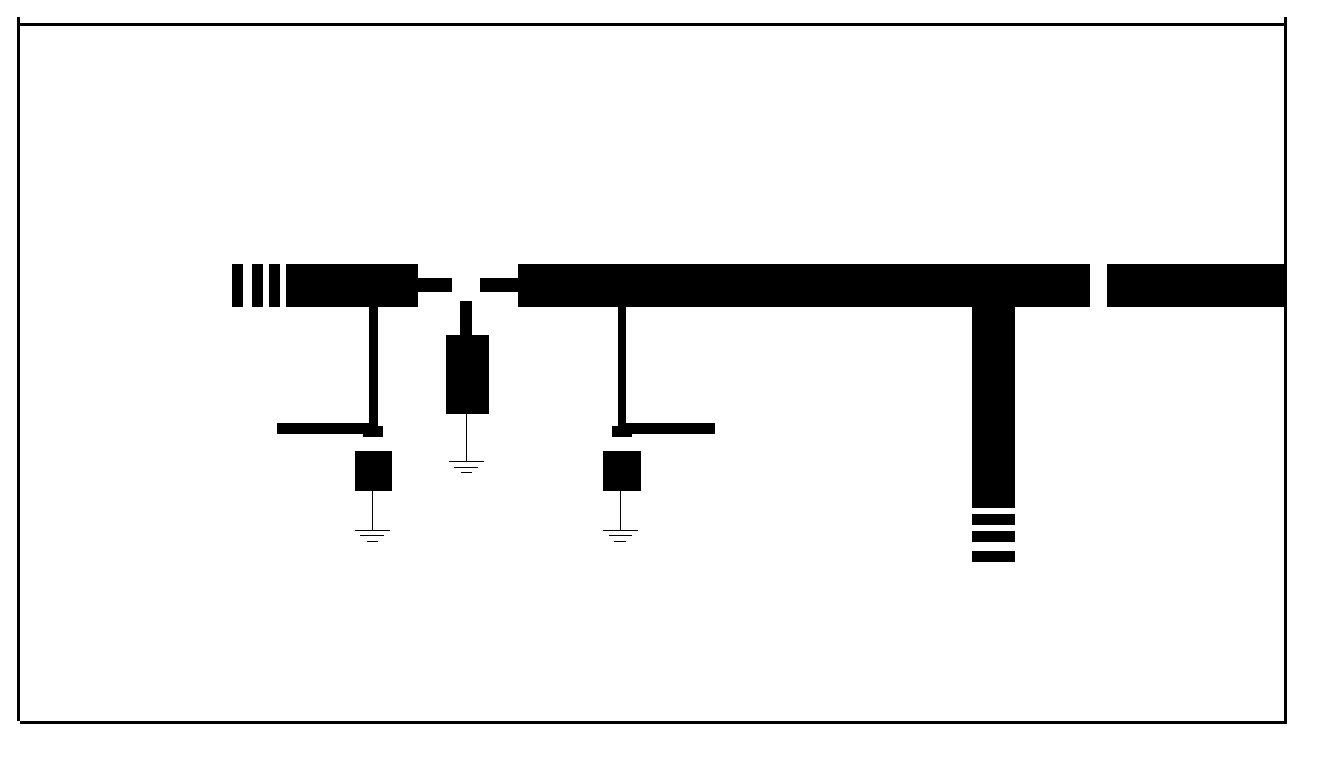
\includegraphics[width=4.79028in,height=2.74931in]{media/image17.png}
\end{quote}

\begin{longtable}[]{@{}l@{}}
\toprule
\endhead
\begin{minipage}[t]{0.97\columnwidth}\raggedright
\begin{quote}
WB:0.3MM\\
WL:2.31MM\\
~\\
*ByPass information\\
CBY:10PF\\
LBY:0.478NH\\
~\\
BLK\\
* Gate Circuit\\
OST 1 W=WL P=4.9MM MSUB\\
TEE 1 2 3 W1=WL W2=WL W3=WB MSUB\\
~\\
* RFC circuit\\
VIA 31 D=1MM MSUB\\
TRL 31 32 W=2MM P=2MM MSUB\\
SRX 32 33 R=0 L=LBY C=CBY\\
TRL 33 34 W=1MM P=0.5MM MSUB\\
OST 34 W=0.5MM P=5.29MM MSUB\\
STEP 34 35 W1=1MM W2=0.3MM MSUB\\
TRL 35 3 W=0.3MM P=7MM MSUB\\
~\\
~\\
TRL 2 41 W=WL P=2.46MM MSUB\\
STEP 41 42 W1=WL W2=0.51MM MSUB\\
TRL 42 4 W=0.51MM P=2MM MSUB\\
~\\
TWO 4 5 6 NE71083\\
~\\
* Source Circuit\\
VIA 61 D=1MM MSUB\\
TRL 61 62 W=WL P=4.45MM MSUB\\
STEP 62 63 W1=WL W2=0.51MM MSUB\\
TRL 63 6 W=0.51MM P=2MM MSUB\\
~\\
* Dran Circuit\\
TRL 5 71 W=0.51MM P=2MM MSUB\\
STEP 71 72 W1=0.51MM W2=2.31MM MSUB\\
~\\
TRL 72 73 W=WL P=5.88MM MSUB\\
TEE 73 74 9 W1=WL W2=WL W3=WB MSUB\\
~\\
* RFC circuit\\
VIA 91 D=1MM MSUB\\
TRL 91 92 W=2MM P=2MM MSUB\\
SRX 92 93 R=0 L=LBY C=CBY\\
TRL 93 94 W=1MM P=0.5MM MSUB\\
OST 94 W=0.5MM P=5.29MM MSUB\\
STEP 94 95 W1=1MM W2=0.3MM MSUB\\
TRL 95 9 W=0.3MM P=7MM MSUB\\
~\\
DRMS 74 10 D=5.9MM HD=2.38MM ER=39 S=2.5MM HT=0.88MM W=WL L=10.6MM BSF
MSUB\\
TEE 10 11 12 W1=WL W2=WL W3=WL MSUB\\
OST 12 W=WL P=11.54MM MSUB\\
TRL 11 13 W=WL P=5.42MM MSUB\\
SRX 13 14 R=0 L=LBY C=CBY ;Chip cap for coupling\\
~\\
OSC:1POR 14\\
~\\
END\\
~\\
FREQ\\
9.99839973449707GHz\\
STEP 2GHz 18GHz 200MHz\\
STEP 9.99GHz 10.01GHz 50KHz\\
END\\
~\\
OUT\\
PRI OSC S\\
END\\
~\\
OPT\\
OSC\\
F=9.99839973449707GHz\\
MS11 W=-1\\
END\\
~\\
~\\
DATA\\
~\\
MSUB : MS ER=2.33 H=0.031in MET1=CU 17.5um\\
~\\
NE71083: S ;Data for NE71083 GaAs MESFET\\
~\\
2GHZ .95 -26 3.54 161 .04 79 .59 -13\\
4GHZ .89 -50 3.1 141 .06 66 .58 -24\\
6GHZ .82 -70 2.83 126 .08 56 .54 -33\\
8GHZ .78 -80 2.49 114 .09 51 .5 -42\\
10GHZ .73 -102 2.15 104 .1 48 .47 -48\\
12GHZ .71 -114 1.95 93 .1 43 .45 -55\\
14GHZ .71 -122 1.93 90 .11 44 .47 -62\\
16GHZ .67 -128 1.64 76 .11 43 .49 -64\\
18GHZ .66 -140 1.47 63 .11 40 .52 -70\\
~\\
END
\end{quote}\strut
\end{minipage}\tabularnewline
\bottomrule
\end{longtable}

\hypertarget{making-a-sample}{%
\section{Making a sample}\label{making-a-sample}}

In the previous chapters, a method to design a TDRO was described and an
optimized circuit was obtained. As the last step, this chapter describes
how to build a unit for testing and measurement.

The PCB circuit is manufactured using PTFE with a specialized fab to
build microwave boards without punching any VIA holes. The VIA holes are
drilled manually using a 1mm drill tip and by using an odd number of
very thin wires, the pads are soldered to the ground plane. Choosing an
odd number of wires helps to assure that the current is distributed
equally and there is a wire in the center of VIA. Five or seven wires
are used for bypass VIA and three wires for transmission lines on the
Source pin of GaAs FET. Soldering must be smooth and monotonous, to
minimize any discontinuities.

The substrate needs to be put inside a chassis with high conductivity.
Brass housing was selected due to its conductivity and easily
solderable. The brass chassis dimensions are selected so that the PCB
becomes flush to one edge and a PCB mounted SMA connector can be screwed
into the chassis. Before putting the PCB inside the chassis, it must be
``washed'' by alcohol, thinner or acetone to make soldering contacts
better. Then using a hot plate, the chassis is heated to the melting
point of solder. Important, is that there should be no open flames
touching brass as it will oxidize it. The back side of PCB must be
coated with soldering paste, for best soldering. Sufficient solder must
be melted inside the chassis to cover it monotonically.

A special attention is needed in melting solder near the hole for the
SMA connector and less solder should be used to not fill the hole. In
the rest of the chassis, there should be enough solder melted that it
covers all the surface but not too much that may overflow once PCB is
placed inside the chassis. Once the PCB is placed inside, the heat
source is removed and the solder joins the PCB ground plane to the brass
chassis generating a ``good'' ground.

DC supplies are connected to the ``fit thru'' bias points outside of the
chassis and to the RFCs inside. Next, the SMA connector is attached and
soldered to the board, followed by the bypass capacitors. As the last
step, the active component, NE71083 is soldered. It needs special
attention that GaAs FET are sensitive to static electricity and heat. To
minimize the chance of damaging it, the solder, soldering iron, and
operator's hands must be connected to ground, by ESD straps. The surface
of the working station must also be grounded for ESD safety. In this
case, the soldering was done on the top of a metal kitchen sink.

Biasing GaAs FET requires two DC supplies for Gate and Drain, which are
calculated below based on the operating point provided by the datasheet.

\[I_{\text{DSS}} = 40mA\]

\[V_{p} = - 1.1v\]

\[V_{\text{DS}} = 3v\]

\[I_{\text{DS}} = 10mA\]

Using the FET current/bias equation:

\[I_{\text{DS}} = I_{\text{DSS}}\left( 1 - \frac{V_{\text{GS}}}{V_{P}} \right)^{2}\]

the Gate bias voltage can be calculated as:

\[V_{\text{GS}} = V_{P}\left( 1 - \sqrt{\frac{I_{\text{DS}}}{I_{\text{DSS}}}} \right)\]

While Source is connected to DC ground, (V\textsubscript{S}=0) the DC
bias supplies are calculated as:

\[V_{G} = - 0.55v\]

\[V_{D} = 3v\]

Time to power up the circuit by connecting the output SMA to a spectrum
analyzer and supplying the DC voltages. First, there is a free-run
oscillation close to 10GHz. Now, manually put DR on its calculated
location. If the circuit stops to oscillate, tune the DR by moving the
conductor plane on the top of the DR until the circuit starts to
oscillate again. The DR can also be moved in regard to the couple
microstrip to best target the oscillation frequency. Once finalized,
glue the DR to the substrate. It is important to use a glue that its
dielectric constant doesn't change after hardening. Before the glue
fully hardens, the last tuning can be done. If needed, increase the
length of open lines to improve the matching.

After building a unit in the lab, the following results were measured:

\begin{quote}
P\textsubscript{0}=9.4 dBm

f\textsubscript{0}=9.998GHz

Z\textsubscript{0}=49.2 Ω (measured using a network analyzer)
\end{quote}

which are very close to the target specifications and approved by the
project advisor.

\begin{quote}
Spring 1998
\end{quote}

\textbf{``That's all folks!''}\footnote{Schneider, Steve. That's All
  Folks! The Art of Warner Bros. Animation. United States, H. Holt,
  1990.}

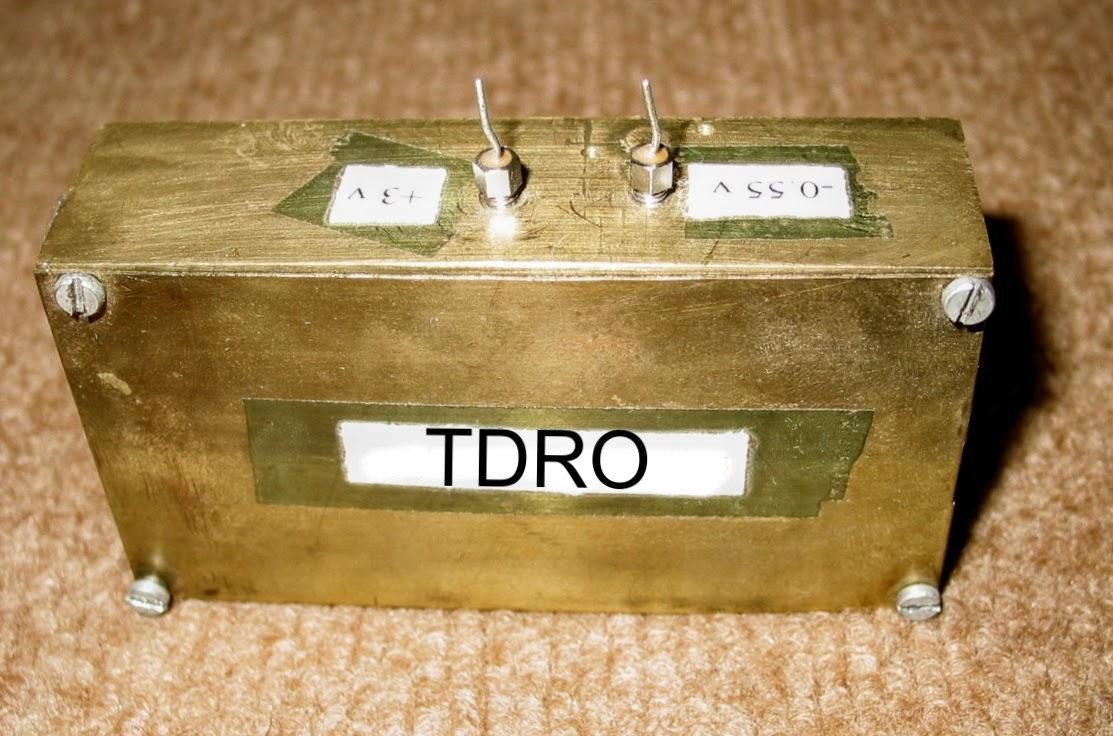
\includegraphics[width=5.20516in,height=3.43912in]{media/image18.jpeg}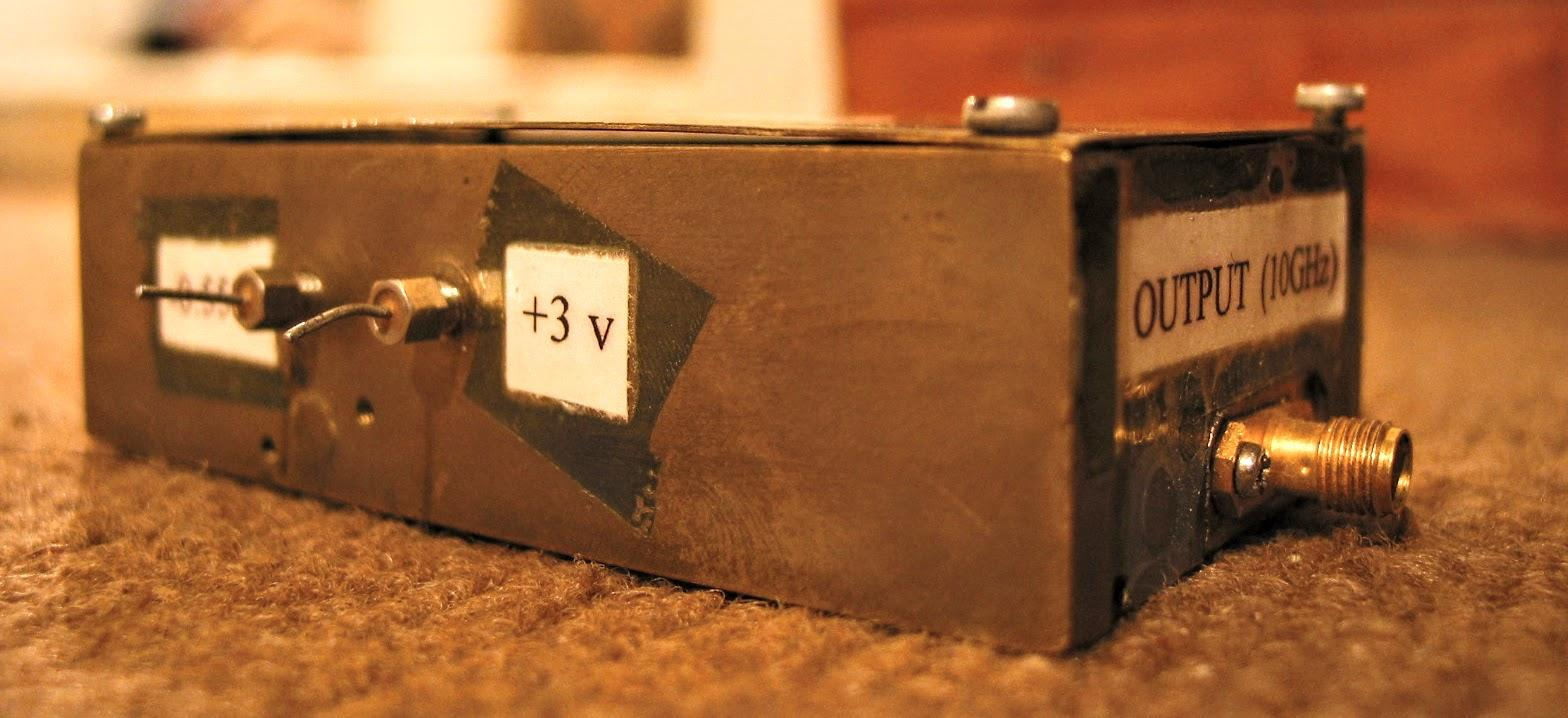
\includegraphics[width=5.21448in,height=2.6417in]{media/image19.jpeg}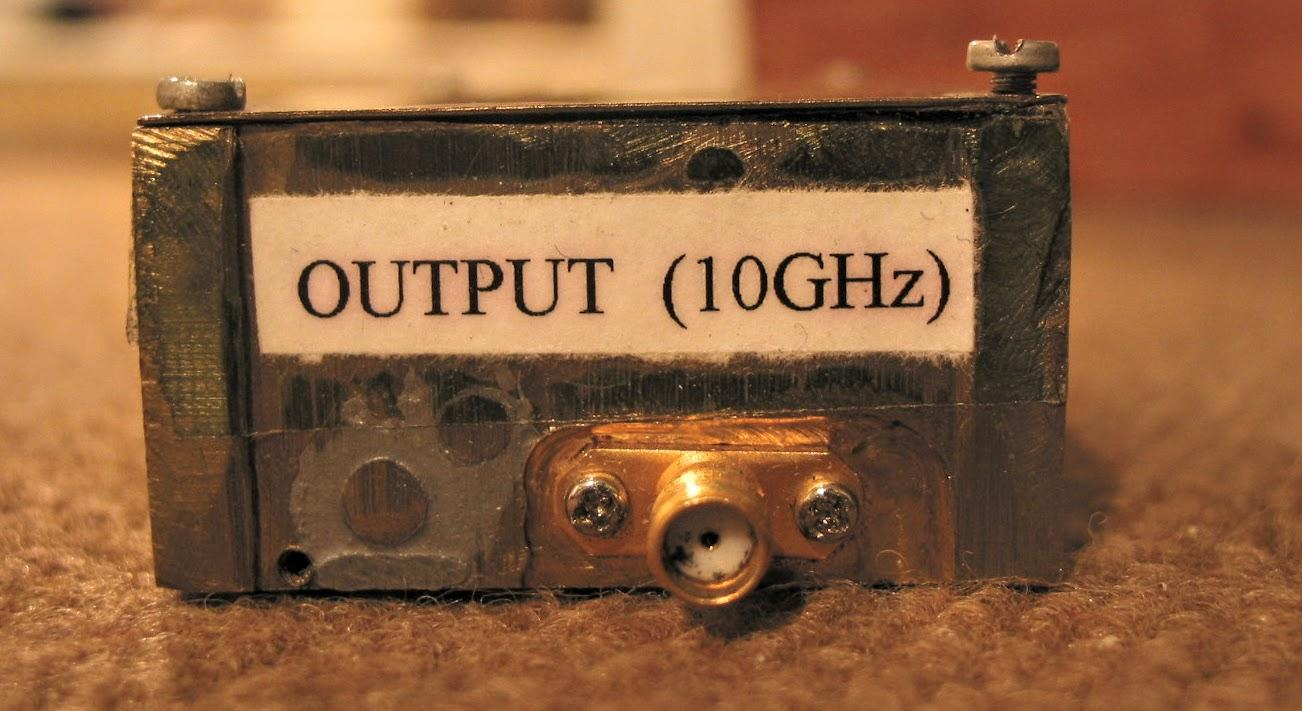
\includegraphics[width=5.22562in,height=2.68768in]{media/image20.jpeg}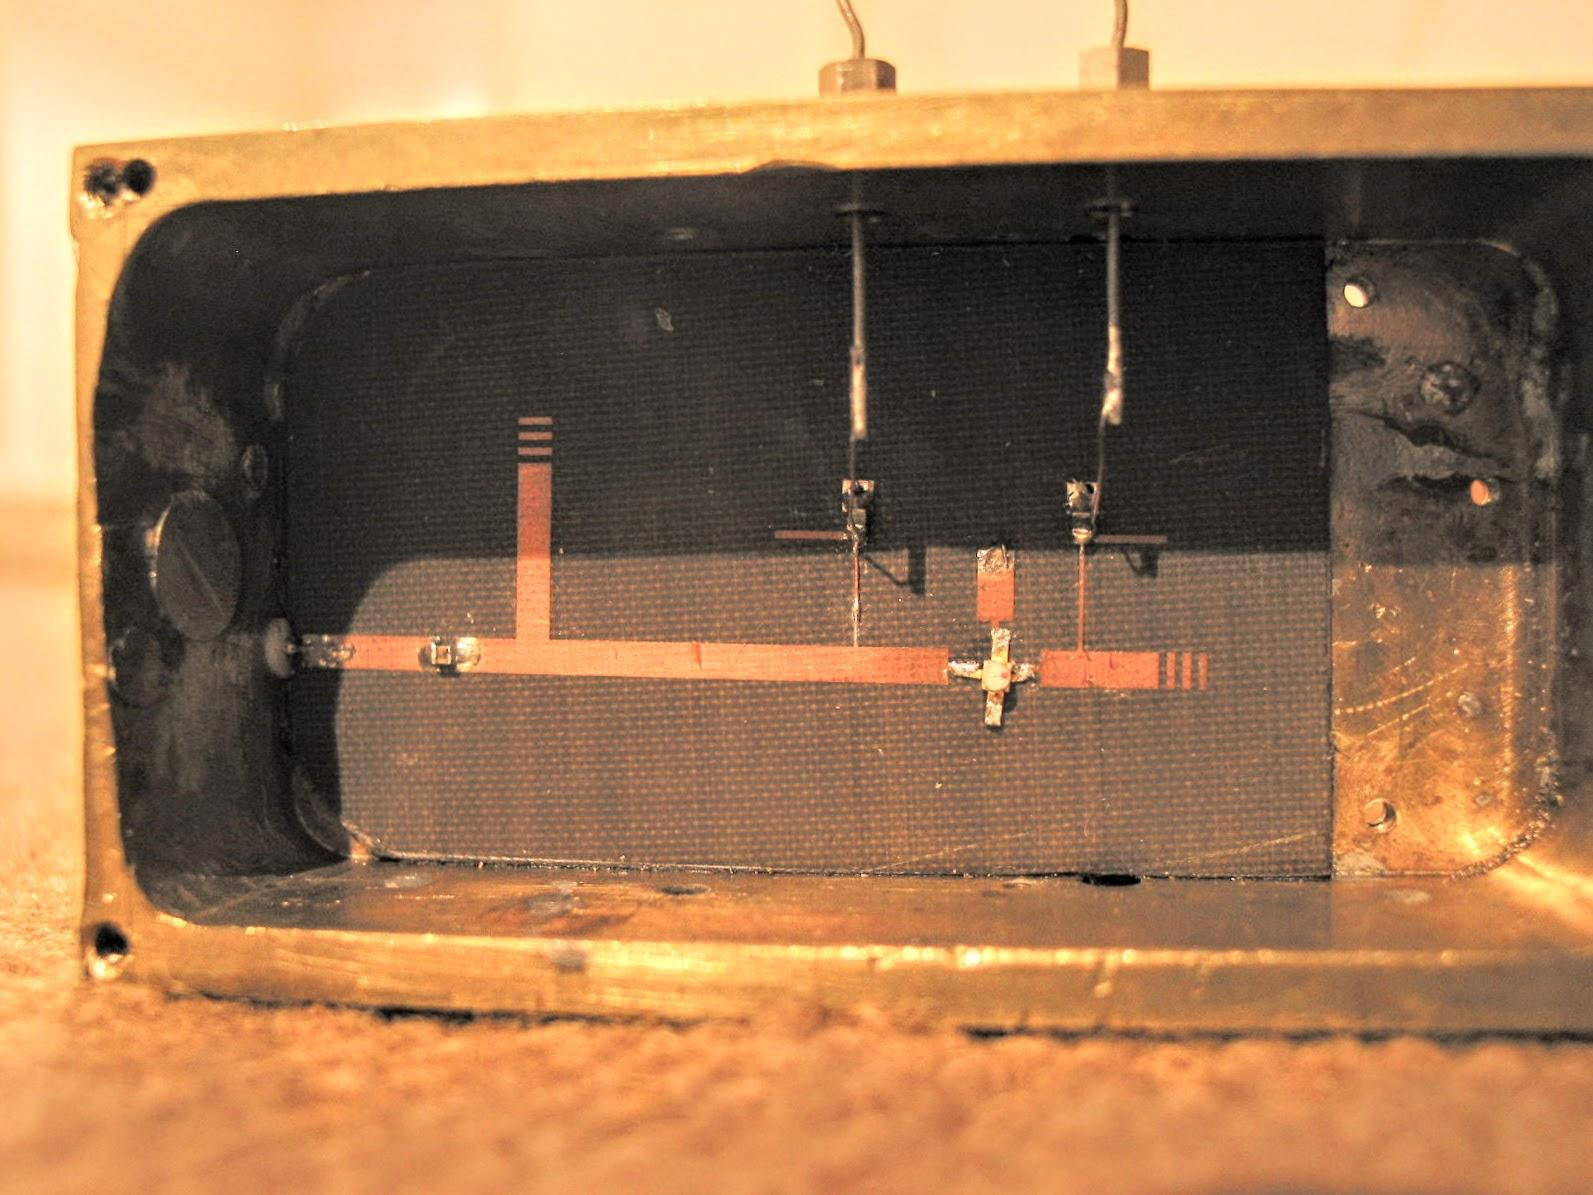
\includegraphics[width=5.16042in,height=3.86757in]{media/image21.jpeg}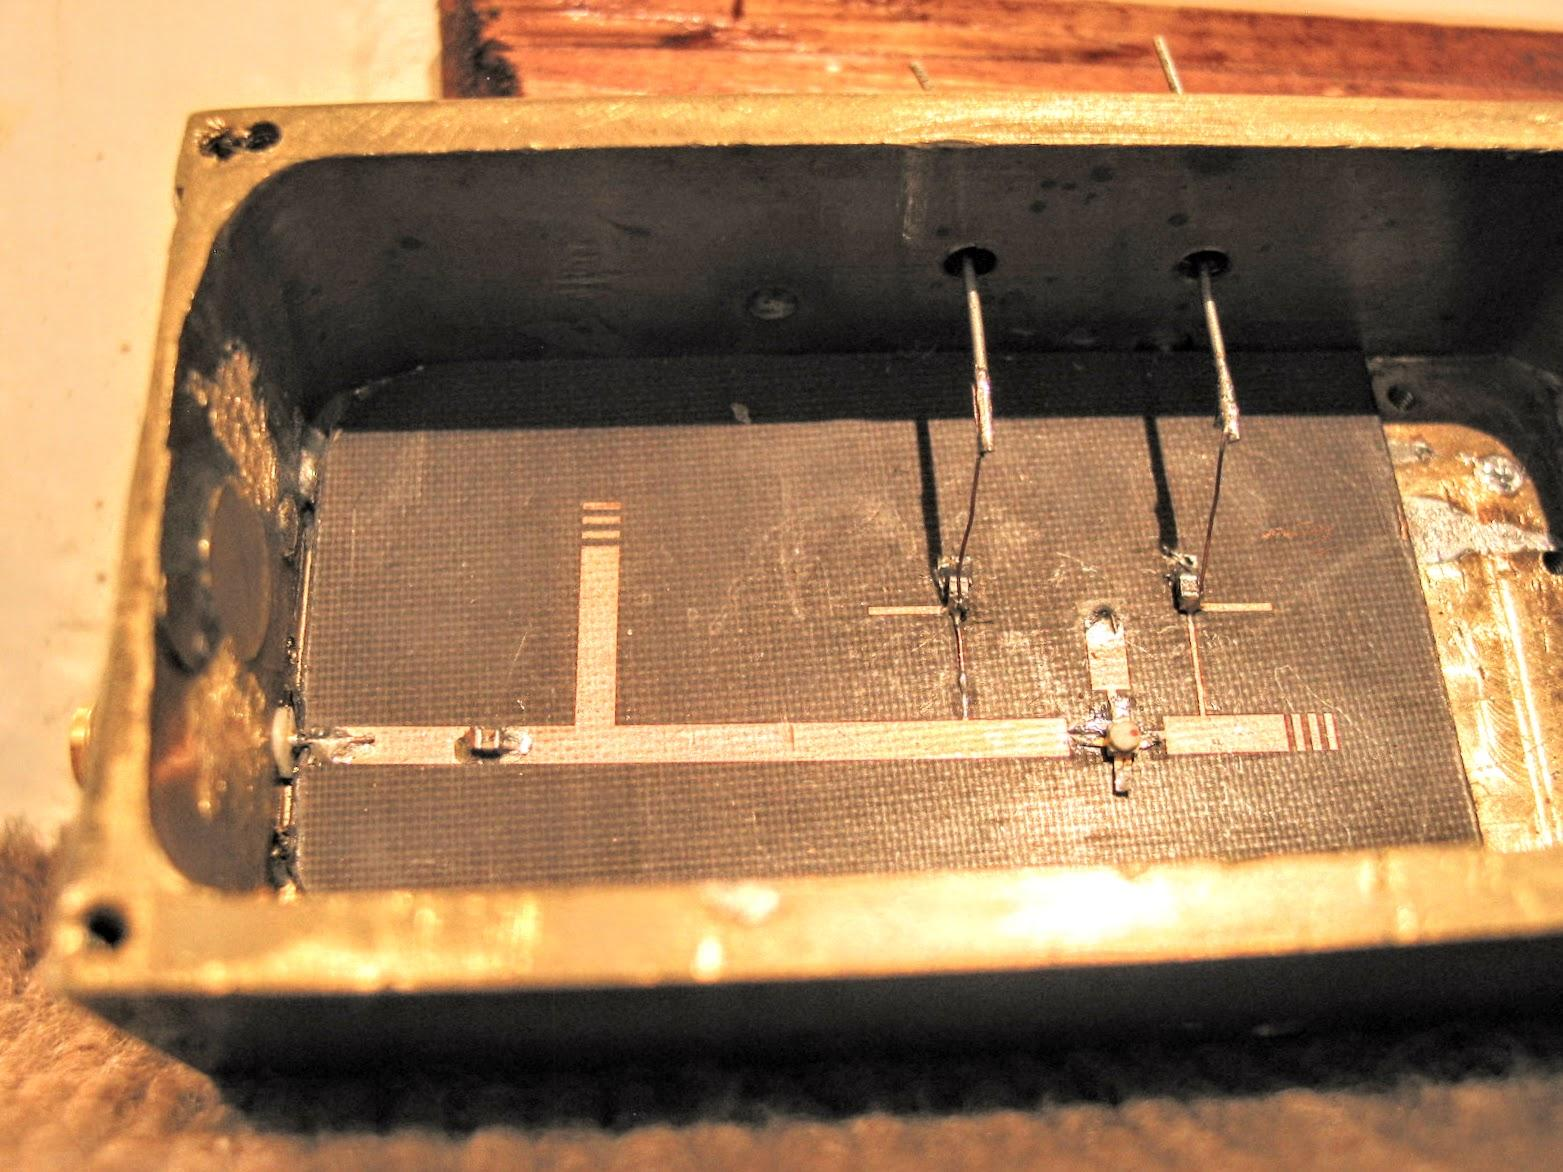
\includegraphics[width=5.13731in,height=3.4864in]{media/image22.jpeg}
